\documentclass[a4paper,12pt]{article}
\usepackage[utf8]{inputenc}
\usepackage[T1]{fontenc}
\usepackage[english]{babel}
\usepackage[nottoc]{tocbibind}
\usepackage{graphicx}
\usepackage{caption}
\usepackage{geometry}
\usepackage{makecell}
\usepackage{adjustbox}
\geometry{a4paper,
             tmargin = 35mm, 
             lmargin = 30mm,
             rmargin = 30mm,
             bmargin = 30mm}
\usepackage{mathtools}
\usepackage{amsmath}
\usepackage{color}
\usepackage{setspace}
\usepackage{amsmath,amssymb}
\usepackage{float}

\usepackage{markdown}
\markdownSetup{
  renderers = {
    link     = {#1},        % Render a link as the link label.
    emphasis = {\emph{#1}}, % Render emphasis using `\emph`.
  }
}

\usepackage{indentfirst}

\usepackage{listings}
\usepackage{afterpage}
\usepackage[font=small,labelfont=bf]{caption}
\pagestyle{plain}

\definecolor{dkgreen}{rgb}{0,0.6,0}
\definecolor{gray}{rgb}{0.5,0.5,0.5}
\definecolor{mauve}{rgb}{0.58,0,0.82}

\lstset{frame=tb,
language=Python,
aboveskip=4mm,
belowskip=4mm,
showstringspaces=false,
columns=flexible,
numbers=none,
keywordstyle=\color{blue},
numberstyle=\tiny\color{gray},
commentstyle=\color{dkgreen},
stringstyle=\color{mauve},
breaklines=true,
breakatwhitespace=true,
tabsize=3
}

\usepackage[hidelinks]{hyperref}

\hypersetup{
  colorlinks   = true, %Colours links instead of ugly boxes
  urlcolor     = blue, %Colour for external hyperlinks
  linkcolor    = blue, %Colour of internal links
  citecolor   = green  %Colour of citations
}

\renewcommand{\thesection}{\Roman{section}.}
\renewcommand{\thesubsection}{\Roman{section}. \arabic{subsection}.}
\renewcommand{\thesubsubsection}{\Roman{section}. \arabic{subsection}.\arabic{subsection}.}

\begin{document}

\linespread{1.5}

\begin{titlepage}

    \centering
    
\includegraphics[width=0.66\textwidth]{elte.jpg}\par\vspace{1cm}
    {\scshape\LARGE Eötvös Loránd University \par}
    \vspace{1cm}
    \rule{140mm}{0.1mm}\\
    \vspace{.5cm}
    {\scshape\Large Scientific imaging \\ using artificial neural networks \\ in medicine\par}
    \vspace{.5cm}
    \rule{140mm}{0.1mm}\\
    \vspace{.5cm}
    {\large\itshape Alex Olar\par}
    \vfill
    supervisor\par
    \vspace{0.5cm}
    {\Large Prof. István Csabai}

    \vfill
    
    {\large 2020 \par}
\end{titlepage}

\begin{abstract}

\vfill

In 2012 a neural network-based architecture won the ImageNet Large Scale Visual Recognition Challenge (ILSVRC) \cite{russakovsky2015imagenet} in object classification. The model was called AlexNet \cite{krizhevsky2012imagenet} named after the creator Alex Krizhevsky. In 2015 a new network from Microsoft Research called ResNet \cite{he2016deep} surpassed human performance in the classification task of ILSVRC and won the Common Objects in Context (COCO) \cite{lin2014microsoft} detection challenge as well. Object localization, segmentation, and image classification since then improved vastly and is still improving to this day. New techniques and state-of-the-arts come out daily and it is extremely difficult to keep up with the surge of scientific papers in computer vision and related fields. This has not remained without attention in biology nor medicine. Computer-aided diagnostics systems have been deployed long before deep learning prevailed but they were ignored or rarely used. As of now, scientists at Google just announced that they have surpassed radiologists in reading mammography images for breast cancer screening \cite{mckinney2020international}, there are ongoing challenges and research for prostate cancer screening as well as stomach cancer screening \cite{li2019signet}. All of these techniques apply some newly emerged computer vision algorithms to enable clinical workers and doctors to work more efficiently and of course to lighten the burden that comes with national screening programs and countless work hours and to advance microscopes as well \cite{chen2019augmented}. In this work, I present results and methods regarding computer-aided diagnostics in colorectal cancer screening that was done collaboratively with Semmelweis University as well as techniques from a project applied to detect glial cells in human brain tissue in collaboration with Semmelweis University and automatic scoring of X-ray images for rheumatoid arthritis (RA2) patients in a Dream Challenge \cite{bionetworks}.

\vfill

\end{abstract}

\newpage

\tableofcontents

\newpage

\section{Introduction}

\vspace{7mm}

\subsection{General}

\vspace{7mm}

Neural networks are universal function approximators that are organized into layers. Layers of a neural network can be highly specialized, such as convolutional layers, that can efficiently learn spatial features, others might simply do matrix multiplication and apply a non-linear mapping to the input to extract underlying information from the data. Neural network architectures nowadays are a concatenation of differentiable layers and training means adjusting the tunable weights of these layers simultaneously based on input data and an objective/loss function that we aim to minimize.

\vspace{4mm}

\par Computer vision for many years was based on hand-engineered feature extraction and although convolutional neural networks (CNNs) were used for some dimensionally constrained problems, such as hand-written digit recognition \cite{lecun1998gradient}. The breakthrough for CNNs came with the advent of graphical processing units (GPUs). As these processors have become widely available due to computer gaming the hardware was pushed to its limits and manufacturers poured a vast amount of money into research. Therefore the GPUs not only did include more on-board memory year-by-year but also performance was improving rapidly. Since computer graphics require a lot of matrix multiplication and concurrent, parallelized computation the scientific community jumped on it and started using graphical processors for general purpose computing.

\vspace{4mm}

\par As computer vision progressed, a need for comparable results was long overdue. The ImageNet Large Scale Visual Recognition Challenge \cite{ILSVRC15} was launched in 2010 with approximately 1.2 million images containing 1000 categories. The goal of the challenge was to classify images into these categories on a held-out test set that was not provided for the participants beforehand. In 2011 a 25\% top-5 error rate was already considered very good but in 2012 the first convolutional neural network-based model \cite{krizhevsky2012imagenet} won the challenge beating the top results by a huge margin. To do so good they used GPUs heavily and proved that image classification is possible via CNNs on large scale images as well. Therefore, the ImageNet top-5 accuracy score became the standard metric of comparing computer vision algorithms and to this day, new architectures are always compared for ImageNet performance in supervised, weakly-supervised and unsupervised settings as well.

\vspace{4mm}

\par Soon after the re-discovery of convolutional networks for image recognition tasks the scientific community in computer vision realized that convolutional neural networks learn generalizable features and the datasets they considered different so far are not so distinct after all. Networks trained on a dataset of recognizing 1000 different classes can be transferred to other datasets with the change of the top of the network to recognize fundamentally different images. This method is called transfer learning and is exceedingly used nowadays thanks to its efficiency. It is rather surprising that a model trained on the ImageNet dataset which contains natural images in different contexts such as dogs in the contry side, cars in traffic, humans at work, etc. can generalize to healthcare applications such as cell segmentation, malignity detection, tissue classification via transfer of these learnt weights. 

\vspace{4mm}

\par Soon enough human performance on ILSVRC was surpassed \cite{he2016deep} by the ResNet architecture and since then people are arguing whether there is still a need for improving ImageNet performance because it is so good. In response to that, the main challenge stopped in 2017 to focus on other problem sets. On the other hand, ILSVRC performance remained a gold standard for architecture evaluation. 

\vspace{7mm}

\subsection{Motivation}

\vspace{7mm}

Currently, deep learning is everywhere and almost everyone is trying to use it to achieve better accuracy in some tasks. In the industry, the main application for artificial intelligence (AI) is to develop self-driving cars in addition to improve recommendation systems for online commercials. On one hand, this certainly drives the economy and as a byproduct we could achieve safer transportation and better overall service as costumers/consumers. On the other hand, it would be highly beneficial for modern society to use computer vision for significantly better healthcare and education. Deep learning has enabled us to do us, from now on, the question is time and effort.

\vspace{4mm}

\par Not so long ago, Google, the tech giant, has partnered with the United Kingdom's healthcare system ( NHS - National Health System ) to gather all the data they can to improve diagnostics and to build algorithms that can work for medics and sanitary workers to improve healthcare. This all sounds too good to be true in capitalism and it is. This has caused outrage amongst the people of the UK \cite{kollewe_2019} regarding personal data protection, however, researchers at Google have some undeniable results such as, reading mammograms better than radiologists \cite{mckinney2020international}, developing a real-time colorectal cancer detection microscope \cite{chen2019augmented}. We are in an era where governments can lead large-scale projects (in data size) to improve their healthcare systems without investing vast amounts of money for equipment, labor and facilities. The COVID-19 crisis showed that with enough data and computational resources pneumonia detection can be achieved with high accuracy \cite{nvidia} proving that computer vision in medicine can be achieved on-demand.

\vspace{4mm}

\par Computer vision has matured enough to reach a state where almost every vision-related task can be done on human performance level or even surpassed by computers. Such as glial cell detection in mouse brain tissue \cite{suleymanova2018deep}, reading mammograms  \cite{ribli2018detecting}, 
predicting colorectal cancer outcome of patients \cite{skrede2020deep}, diagnosing volumetric data such as CT's \cite{cciccek20163d}. I could also mention advancement in weak-lensing, astrophysics \cite{ribli2019improved} and new areas to explore, such as Hamiltonian \cite{greydanus2019hamiltonian} and Lagrangian \cite{cranmer2020lagrangian} neural networks for physics, where the dynamics of the system is deduced from sensory input going so far as learning actual physics from images with generative models \cite{toth2019hamiltonian}. It is also worth to mention advancement in reinforcement learning that started with playing Atari games \cite{mnih2013playing} successfully and on-par with human players and led to playing Dota 2 and Starcraft \cite{alphastarblog} in top-tier leagues, both of which are tremendously complex environments that resemble real world complexity. This might sound irrelevant but reinforcement learning robots will take over the majority of production line jobs \cite{satariano_metz_2020} very soon.

\vspace{4mm}

\par As a consequence, it is high time to research the widespread applications of AI in the medical field and in natural sciences in general. Finally, I am certain that doing something here is highly beneficial not only for self-advancement or other opportunistic reasons but also for society. We are building the future and even though I laid out a rather over-optimistic view on it, we must take precautions while deploying such systems to avoid built-in bias in our models \cite{amodei2016concrete}.

\newpage

\subsection{Overview}

\vspace{7mm}

\par In the following sections I provide a brief overview of what machine learning is and how it is used in computer vision. I gather the intuitions of building such systems and talk more about convolutional algorithms. Also in this section I give a quick walk-through of a simple binary classification problem and show how that can be solved either by logistic regression or via neural networks. Closing this section the general structure of convolutional neural networks is presented.

\vspace{4mm}

\par In the succeeding section, I present in a nutshell the field of medical imaging and especially cancer detection/recognition. Here I mention some statistical details about cancer and demonstrate how computer vision can revolutionize treatment and patient care.

\vspace{4mm}

\par Moving on to the first application that I have been part of for almost a year. In this thesis, I display the techniques we used for different types of colorectal tissue recognition and malignity detection. In addition, I also exhibit the process of gathering a unique and in-size unprecedented dataset for colorectal cancer research and reveal some of our results.

\vspace{4mm}

\par Furthermore, I shortly talk about an on-going DREAM Challenge \footnote{'The DREAM Challenges are an open science effort, a non-profit, collaborative community effort consisting of contributors from across the research spectrum including researchers from universities; technology companies like IBM Research; not for profits, like Sage Bionetworks; and biotechnology and pharmaceutical companies.' - source \url{dreamchallenges.org/about-dream}} that deals with automated rheumathology. As the competition is still in progress, I cannot disclose any data, not even for presentation, nor include any results, as a consequence I only present our work and the methods we used. Currently we are amongst top participants.

\newpage

\section{Computer vision}

\vspace{7mm}

\subsection{Vision}

\vspace{7mm}

\par The human visual cortex is composed of many hierarchical layers. The image data required by our eyes is processed through cells on the retina that are sensitive to light known as the rods and cones. The rods are sensitive to color whilst the cones are sensitive to the intensity of the photons. The number of cones is significantly higher than the number of rods, therefore we are much more adapted to detecting light intensity than to colors. There are three types of these cone cells causing trichromacy \cite{arrese2002trichromacy} and therefore in computer science, the most widespread format of storing image data is in RGB (red-green-blue) channels. The visual cortex is doing edge detection in the V1 (primary visual cortex) which has been computationally reproduced \cite{olshausen1996emergence} while it is assumed that the V2 \cite{ZiembaV2} and V4 are doing much more abstract representations, the latter already producing objects. Some researchers are occupying with demonstrating the same in neural networks \cite{cammarata2020thread:}.

\vspace{4mm}

\begin{minipage}[t]{0.35\textwidth}
    \centering
    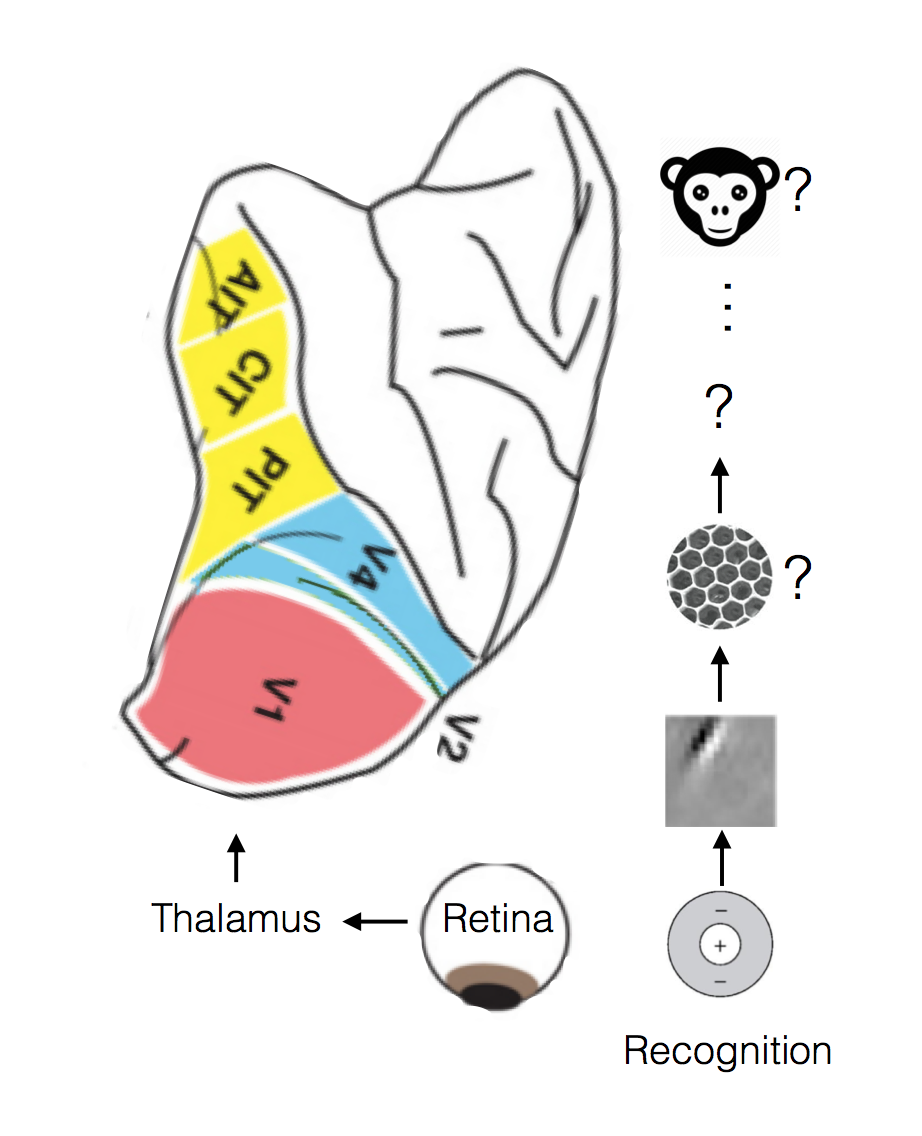
\includegraphics[width=\textwidth]{intro/visual-cortex.png}
    \captionof{figure}{General layout of the human visual cortex}
    \label{fig:human-cortex}
\end{minipage}
\begin{minipage}[t]{0.55\textwidth}
    \centering
    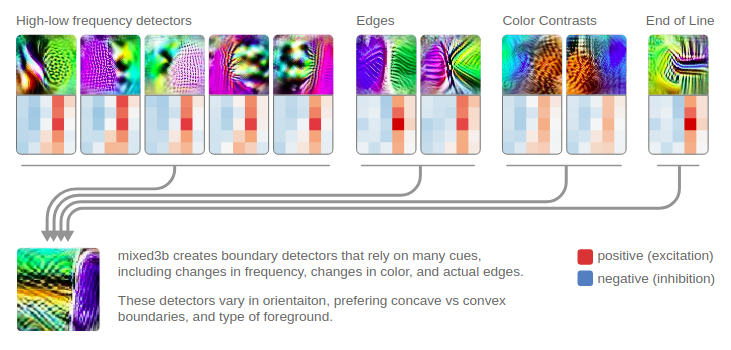
\includegraphics[width=\textwidth]{intro/eraly-vision-distill.png}
    \captionof{figure}{Early vision in a convolutional neural network - source \url{https://distill.pub/2020/circuits/early-vision/}}
    \label{fig:sigmoid}
\end{minipage}

\vspace{7mm}

\subsection{Convolutional neural networks}

\vspace{7mm}

\par All these arguments inspired many-layered convolutional neural networks that are doing computations on spatial data such as images. Convolutions are about learning sliding kernels on three-dimensional image data (two spatial dimensions and color channels, 2 + 1) these kernels provide efficient and translation invariant parameters for the models. The convolutional operation is relatively simple and straight-forward. On one dimensional sequences and functions, it is defined as:

\begin{align*}
    (u * v)_n = \sum_{m = -\infty}^{\infty} u_{m} v_{n-m} \\
    (f * g)(t) = \int_{-\infty}^{\infty} f(\tau)g(t-\tau)d\tau
\end{align*}

\vspace{4mm}

\par Spatially this is defined similarly but for a finite $K$ kernel with size $(k_1, k_2)$:

\vspace{4mm}

\begin{align*}
    (I * K)_{ik} = \sum_{m = 1}^{k_1}\sum_{n = 1}^{k_2} I_{i - m, k - n} K_{m, n}
\end{align*}

\vspace{4mm}

\par This can be visually illustrated by the figure below where the parameters of $K$ (blue) are learned algorithmically by seeing lots of examples:

\vspace{4mm}

\begin{figure}[H]
    \centering
    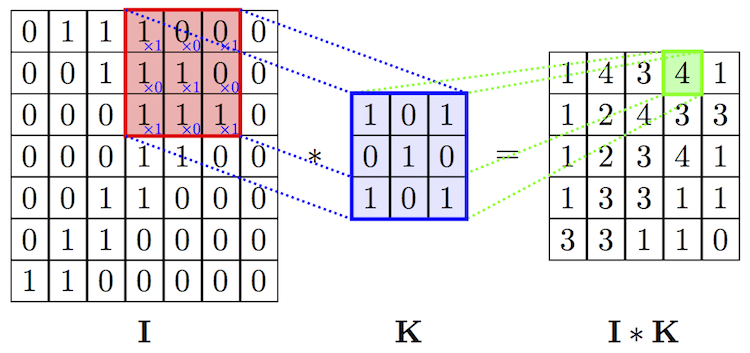
\includegraphics[width=0.7\linewidth]{An-example-of-convolution-operation-in-2D-2.png}
    \caption{2D convolution - Scientific Figure on ResearchGate. Available from: \url{https://www.researchgate.net/figure/An-example-of-convolution-operation-in-2D-2_fig3_324165524} [accessed 31 Mar, 2020]}
    \label{fig:2d-conv}
\end{figure}

\vspace{4mm}

\par There are two main branches of machine learning, such as supervised and unsupervised learning. In applications of computer vision supervised learning is used most of the time as it is more interpretable than unsupervised techniques and generally the goal of unsupervised learning is pre-training for supervised algorithms or knowledge distillation. These are methods for image classification, object detection/segmentation. These all work by defining an objective function we want to minimize to achieve a desired rate of error. 

\vspace{4mm}

\par The difference between a traditional regression method and a neural network lies in the fact the we aim to develop algorithms that generalize extremely well on unseen data, therefore we not solely aim to minimize the objective function on our data but to do so on every possible dataset that comes from the same underlying distribution. To achieve this the standard way of developing these algorithms is to split any dataset to training, validation and testing sets where we validate our algorithms on the validation set, tuning the parameters during training in order to achieve the low validation error then, without modification we evaluate on the test set. This is necessary since by tuning hyper-parameters of training we inherently minimize error on the validation set, therefore tuning for validation performance which is biased. The gap between validation error and test error somehow measures the rate of this bias and the aim is to keep this minimal.

\subsubsection{Binary classification}

\vspace{4mm}

\par The simplest case of supervised learning is probably binary classification. In binary classification we want to maximize the joint probability of getting a data point $x$ and by applying a function $f(x, \theta) = \hat{y}$, where $\theta$ are function parameters, we predict $\hat{y}$ probability for $x$ being in class $1$ and therefore $1 - \hat{y}$ probability for being in class $0$. If $y$ is the true label of the data point, then we can formalize our explanation as:

\vspace{4mm}

\begin{align*}
    P(y = 1 | x) = \hat{y} \\
    P(y = 0 | x) = 1 - \hat{y} \\
    \quad \rightarrow P(y | x) = \hat{y}^{y} \cdot (1 - \hat{y})^{(1-y)}
\end{align*}

\vspace{4mm}

\par We want to maximize the sum of this joint probability for all the examples we have in a dataset but we can do so by taking the logarithm of this since the logarithm function is bijective. We call this our objective or loss function we aim to minimize:

\vspace{4mm}

\begin{equation}
    L\big(y, \hat{y}\big) = -\sum_{i = 1}^{N_{data}} \Big(y^{(i)}\log\hat{y}^{(i)} + (1 - y^{(i)})\log(1 - \hat{y}^{(i)})\Big)
    \label{eq:bernoulli-loss}
\end{equation}

\vspace{4mm}

\par In this special case (\ref{eq:bernoulli-loss}) is called the Bernoulli-loss, due to the binary variable we predict. As we acquired $\hat{y}^{(i)}$ as a function $f(x^{(i)}, \theta) = \hat{y}^{(i)}$ on the data point $x$ with parameters $\theta$, therefore the objective function is parametrized by $\theta$ as well. 

\vspace{4mm}

\par The simplest technique would be to do linear regression on the training data and normalize it to $(0, 1)$ with a sigmoid function. This is called logistic regression and can be done by fitting the data to the objective with familiar methods or with gradient steps as described in the next paragraph.

\vspace{4mm}

By feeding exemplary data points to $f$ and calculating the loss we could also calculate the corresponding derivatives of the loss to the parameters $\frac{\partial L}{\partial \theta}$ and apply these derivatives with a predefined rate $\mu$ to improve the objective. We call this gradient descent since the gradient of the function gives the biggest slope on the multidimensional surface spanned by $\theta$ and if we move to the opposite direction of the gradients we then minimize the desired function. We call it batch stochastic gradient descent (SGD) if only a batch of samples is used due to computational resource limitations. This introduces noise to the learning process but if we sample the data uniformly we could still improve the objective function in many iterations:

\vspace{4mm}

\begin{equation}
    L_{batch} = - \sum_{\#batch\_size}L(y^{(i)}, \hat{y}^{(i)}) = L_{batch}(\theta)  
\end{equation}

\vspace{4mm}

\par The gradient with respect to (w.r.t) $\theta$ can be applied with batch SGD in the update step after each sample of data points:

\vspace{4mm}

\begin{equation}
    \theta = \theta - \mu \frac{\partial L}{\partial \theta}
\end{equation}

\vspace{4mm}

\par As it is evident from above any type of differentiable objective function can be used with any differentiable model $f$ and the model can be trained on samples of the dataset to yield a successful predictor for previously unseen data points. Computer vision aims to be able to generalize algorithms as much as possible. The success of deep learning and convolutional neural networks lies in generalization since with large enough datasets they have a very close performance on unseen data as on training data. Therefore we could train a model to recognize lung damage on CT scans on a large enough dataset and apply it in every hospital in the world where they have a gaming graphics card. This solution is feasible and can improve healthcare tremendously. For lower-risk applications, it is even possible to run models in the browser using WebGL technology that recognizes the graphics capabilities of the underlying machine and uses it to run trained models \cite{cohen2019chester}.

\vspace{4mm}

\subsubsection{Structure of a modern CNN}

\vspace{4mm}

\par The structure of a modern convolutional neural network is the following: the input is a 3-dimensional array, representing an image. The image is then fed-forward through convolutional layers with different sized and multiplicity of filters. The main intuition behind selecting the right filter/kernel sizes comes from the VGG16 architecture \cite{simonyan2014very}. This intuition is that small kernels, usually $3x3$, can have a high receptive field after many layers, therefore using larger kernels only uses more computational resources and not that useful after all. Since the image is compressed after convolutions by maximum or average pooling or strided convolutions it is usually so that the number of kernels used is increased with the spatial size of the input image is decreased. After convolutional layers, the data is flattened into a vector or each feature map gets globally maximum or average pooled and fed into a multi-layer perceptron which is matrix multiplications followed by non-linearities \ref{fig:modern-cnn}.

\vspace{4mm}

\begin{figure}[H]
    \centering
    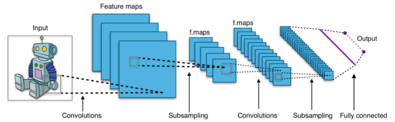
\includegraphics[width=.8\linewidth]{wiki_cnn.png}
    \caption{Structure of a convolutional neural network - Convolutional neural networks, Wikipedia}
    \label{fig:modern-cnn}
\end{figure}

\vspace{4mm}

\par The non-linearities or activation functions are applied after each layer to make the computation non-linear. This is necessary since a sequence of linear computations can always be replaced by a single matrix multiplication. The best working non-linearity proved to be the rectified linear unit, ReLU,  in deep learning and is used throughout many networks. The last non-linearity, on the other hand, can be different based on the problem. For regression, it might not be needed with unbounded predictions, for binary classification the sigmoid function is used which saturates the real numbers to the $(0, 1)$ interval and for non-binary classification the softmax function is used which returns a probability distribution over N classes for each input. The computations are done in batches, as everything is parallelizable, computation can be sped up by the number of available processor units, shared memory is only needed for the final loss computation.

\vspace{7mm}

\begin{minipage}[t]{0.45\textwidth}
    \centering
    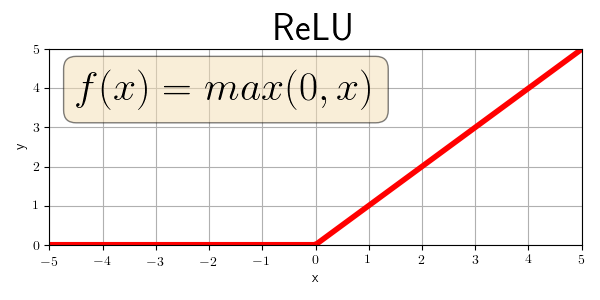
\includegraphics[width=\textwidth]{relu.png}
    \captionof{figure}{Rectified linear unit}
    \label{fig:relu}
\end{minipage}
\begin{minipage}[t]{0.45\textwidth}
    \centering
    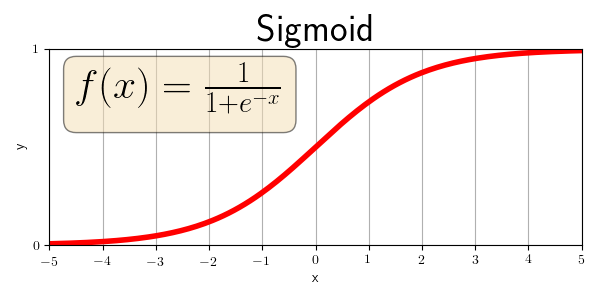
\includegraphics[width=\textwidth]{sigmoid.png}
    \captionof{figure}{Sigmoid}
    \label{fig:sigmoid}
\end{minipage}

\vspace{4mm}

\begin{equation}
    softmax(\vec{x}) = \frac{e^{\vec{x}}}{\sum_{i}e^{\vec{x}_i}}
\end{equation}

\vspace{4mm}

\par We have seen the objective function for binary classification before where we use the sigmoid activation function to acquire probabilities from the model but in the case of multi-class, mutually-exclusive labels we use the cross-entropy loss that is defined as:

\vspace{4mm}

\begin{equation}
    L_{CE} = - \sum_{i = 1}^{N_{class}} y_{i}\log\hat{y_{i}}
\end{equation}

\vspace{4mm}

\par For multi-object detection and segmentation much diverse and more intricate loss functions are used and the networks themselves \cite{ren2015faster} are modified as well to handle sliding-windows efficiently via convolutions \cite{redmon2016you}. I present these in the section of rheumathology automation since we use object localization networks in that setting and it is not closely linked to the general definition of convolutional networks.

\newpage

\section{Medical imaging}

\vspace{7mm}

\par Medical imaging was a thing since the discovery of the X-ray. In the beginning, as in photography, they used light-sensitive materials to capture the different amounts of radiance from the light source but as everything became digitized in the 20th century the field moved on to using silicon-based sensors. These capture data that can be converted to pixel values and used by the computer. Some kind of image processing is inevitable due to contrast, brightness, hue, and other corrections such as image stabilization for moving objects.

\vspace{4mm}

\par In medicine and biology, a fast digitization process can be experienced. Even in Hungary clinics are starting to realize that the future is based on digital processing of biological samples. Some techniques were inherently digital such as MRI \footnote{magnetic resonance imaging} and fMRI \footnote{functional-MRI} and PET \footnote{positron emission tomography} due to the process involved requiring the image, however, in pathology where a large number of biopsies are taken each year the case is not so. Medics usually scan to manually sliced slices of tissue via optical microscopes and make decisions based on that. This method works well and is reliable but does not scale well. 

\vspace{4mm}

\par There exist many companies that manufacture digital microscopes that can process many slides of tissue samples a day and save high-quality images to a local, clinical database. With the advent of deep learning, this data can be pre-processed via computer vision algorithms. It is only a matter of proper data acquisition by the clinical institutes to enable large scale applications such as automatized negative case dismissal, cell count in any kind of tissue, alerts on maligns cases, and even improved diagnostic capabilities.

\vspace{7mm}

\subsection{Cancer detection}

\vspace{7mm}

\par Reading mammograms and evaluating tissue samples for colorectal cancer takes years of practice after acquiring a degree in medicine. The skill is gathered by seeing many samples and noticing little but usual similarities between different patients. 

\vspace{4mm}

\par For mammography, the image is an X-ray scan of the tissue, and noticing nodules is the goal. In Hungary and also in the UK it is mandatory for a medic after finishing university to obtain a certificate for reading mammograms since it is not a trivial thing to do well. On the other hand, there are countries where this is not required and it shows in performance, which is shown in \cite{mckinney2020international}.

\vspace{4mm}

\par For pathologist the tissue is usually stained with H\&E \footnote{haemotoxylin and eosin} staining, which is a standard protocol \cite{fischer2008hematoxylin}, that has a specific purple and pink color. Inspecting these through microscopes enables doctors to issue diagnosis based on the visual attributes of the samples.

\vspace{4mm}

\par Since it seems that cancer detection in such tissue is mainly based on visual attributes of the environment it should not be surprising that the task can be done with convolutional neural networks.

\vspace{4mm}

\par According to the WHO \footnote{World Health Organization} every one death out of six is due to cancer \cite{whoCANCER}. The leading cancer type among women is breast cancer while it is colorectal cancer in men. We disregard here the large case number of lung cancer since it is mainly due to smoking and is in decay for decades now.

\vspace{4mm}

\begin{figure}[H]
    \centering
    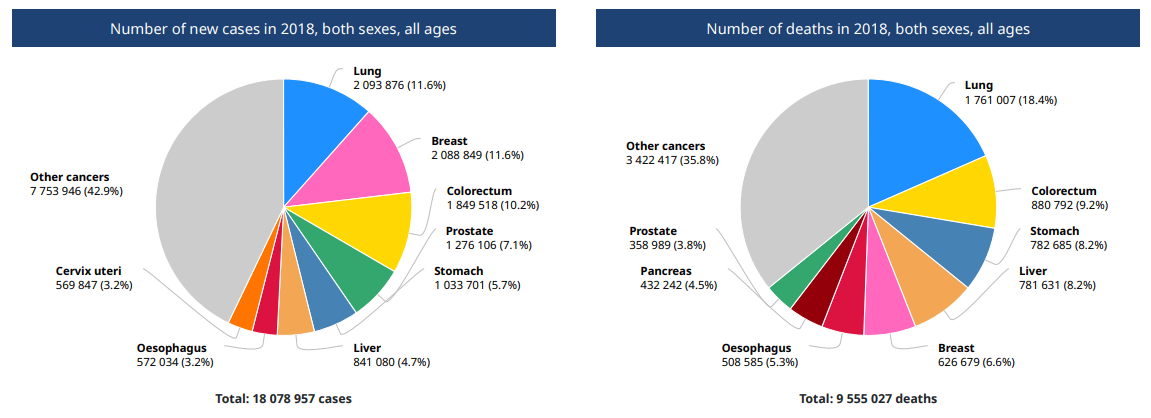
\includegraphics[width=0.8\textwidth]{all_cancer_pie_charts.png}
    \caption{New cancer cases and death rates according to the International Agency on Cancer Research,  WHO}
    \label{fig:cancer_pie_chart}
\end{figure}

\vspace{4mm}

\par The lower than expected death rate in breast cancer is due to the national screening programs that can detect malign lesions before they are in a terminal state. National colorectal cancer screening programs have been launched in the past decade in the Netherlands \cite{rivm_2014}, in the UK \cite{gov.uk_2015} and are rolling out or in an early stage in many other countries according to the European Union \cite{euReportOnCancer}.

\vspace{4mm}

\par A national screening program requires a lot of effort from the pathologist and much more highly-skilled working hours that are available in any country. It cannot be a short-term solution to educate more doctors in this skill for obvious reasons, therefore we should turn to other available solutions. One is to automate as many things as possible. For screening programs, a huge impact can be achieved by dismissing negative samples and only letting through positive ones with extremely high precision and crucially low false-negative rate. On the other hand, one might be interested in pre-selecting high-risk patients based on the diagnosis to start treatment as soon as possible.

\newpage

\section{Deep learning in pathology}

\vspace{7mm}

\par In the project we have been working on in collaboration with the 2nd Department of Pathology- Semmelweis University we aimed to collect a large amount of digitized whole slide scans from rectal biopsies and annotate them with an expert pathologist. The annotation process included global labels and local, free-hand area annotations for specific lesions. Having acquired the necessary amount of data we developed and validated a sophisticated autonomous detection system via computer vision techniques. We qualitatively compare the AI pathologist with human experts in all categories.

\vspace{4mm}

\subsection{Screening process}

\vspace{4mm}

\par The screening process involves the following steps: first a surgeon takes a sample from the bowel of the patient and he/she sends it to histology where pathologists analyze and diagnose the sample. We use these digitized samples to make a diagnosis with the autonomous system.

\vspace{4mm}

\subsection{Similar studies}

\vspace{4mm}

\par Many studies have emerged in the past few years using modern computer vision techniques in biomedical imaging and bowel tissue analysis is not an exception at all. One of the first studies occupied with rectal polyp classification \cite{korbar2017deep}, while another study extract features with a deep network trained on natural images and uses those features to predict a more precise grade for the COAD WSI \footnote{Colon Adenocarcinoma Whole Slide Imaging} data \cite{bychkov2018deep}. A recent study similar to ours shows \cite{skrede2020deep} survival probability based on whole slide images.

\vspace{4mm}

\subsection{Goals}

\vspace{4mm}

\par There are a few distinct ways of handling large scale whole slide images. Usually in deep learning images are sized less than \begin{markdown}
`1024 x 1024 x 3`
\end{markdown} 
pixels and therefore one can cut out small pieces of a large image and train a network on that data to classify the patches, this was done by \cite{korbar2017deep}, \cite{bychkov2018deep} and \cite{skrede2020deep}. It is also possible to extract features from these smaller patches and then put together those as training data for a new network to classify the whole image in its integrity for something, this was done by \cite{skrede2020deep} and we have a very similar approach but not for survival but total whole slide patch level segmentation of the image. We aim to categorize every patch and draw a diagnosis based on the full slide. To make our diagnoses interpretable we need to categorize every region as a human would do and give back localized information and reduce that to diagnosis later on. Our work is also very similar to \cite{takahama2019multi} since we use a two-step prediction process to acquire higher accuracy.

\vspace{4mm}

\subsection{Data}

\vspace{4mm}

\par The tissue segments were scanned at 400x zoom and annotated with the QuPath v0.1.2. software. The software included a viewer and a free-hand ROI \footnote{region of interest} annotator tool but I needed to write a plugin to extract the annotation data. This open-source plugin was developed in Java and is available at \url{https://github.com/qbeer/qupath-binarymask-extension}. The extension is capable of extracting and loading annotation masks from a pre-specified directory into a QuPath project. The annotation mask is saved into PNG format in black and white for efficiently storing and in reduced size based due to very annotated regions.

\vspace{7mm}

\begin{minipage}[t]{0.4\textwidth}
    \centering
    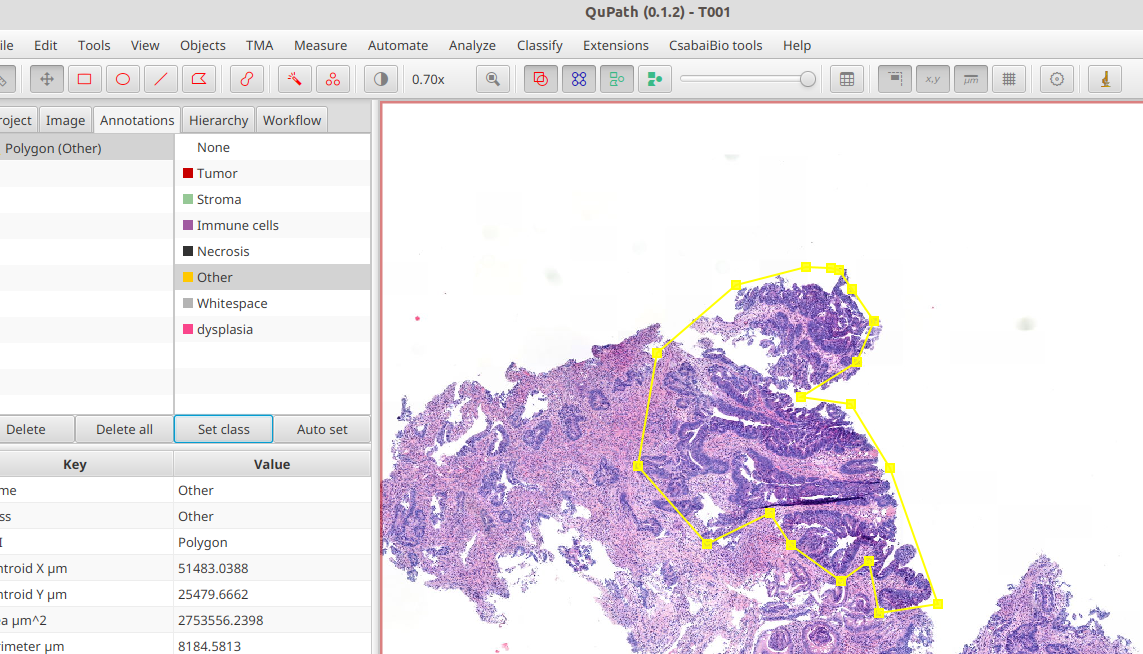
\includegraphics[width=\linewidth]{qupath_screenshot.png}
    \captionof{figure}{View of the annotated region in QuPath, all the metadata saved in the filename of the annotation}
    \label{fig:annotation_qupath}
\end{minipage}\qquad\qquad
\begin{minipage}[t]{0.4\textwidth}
    \centering
    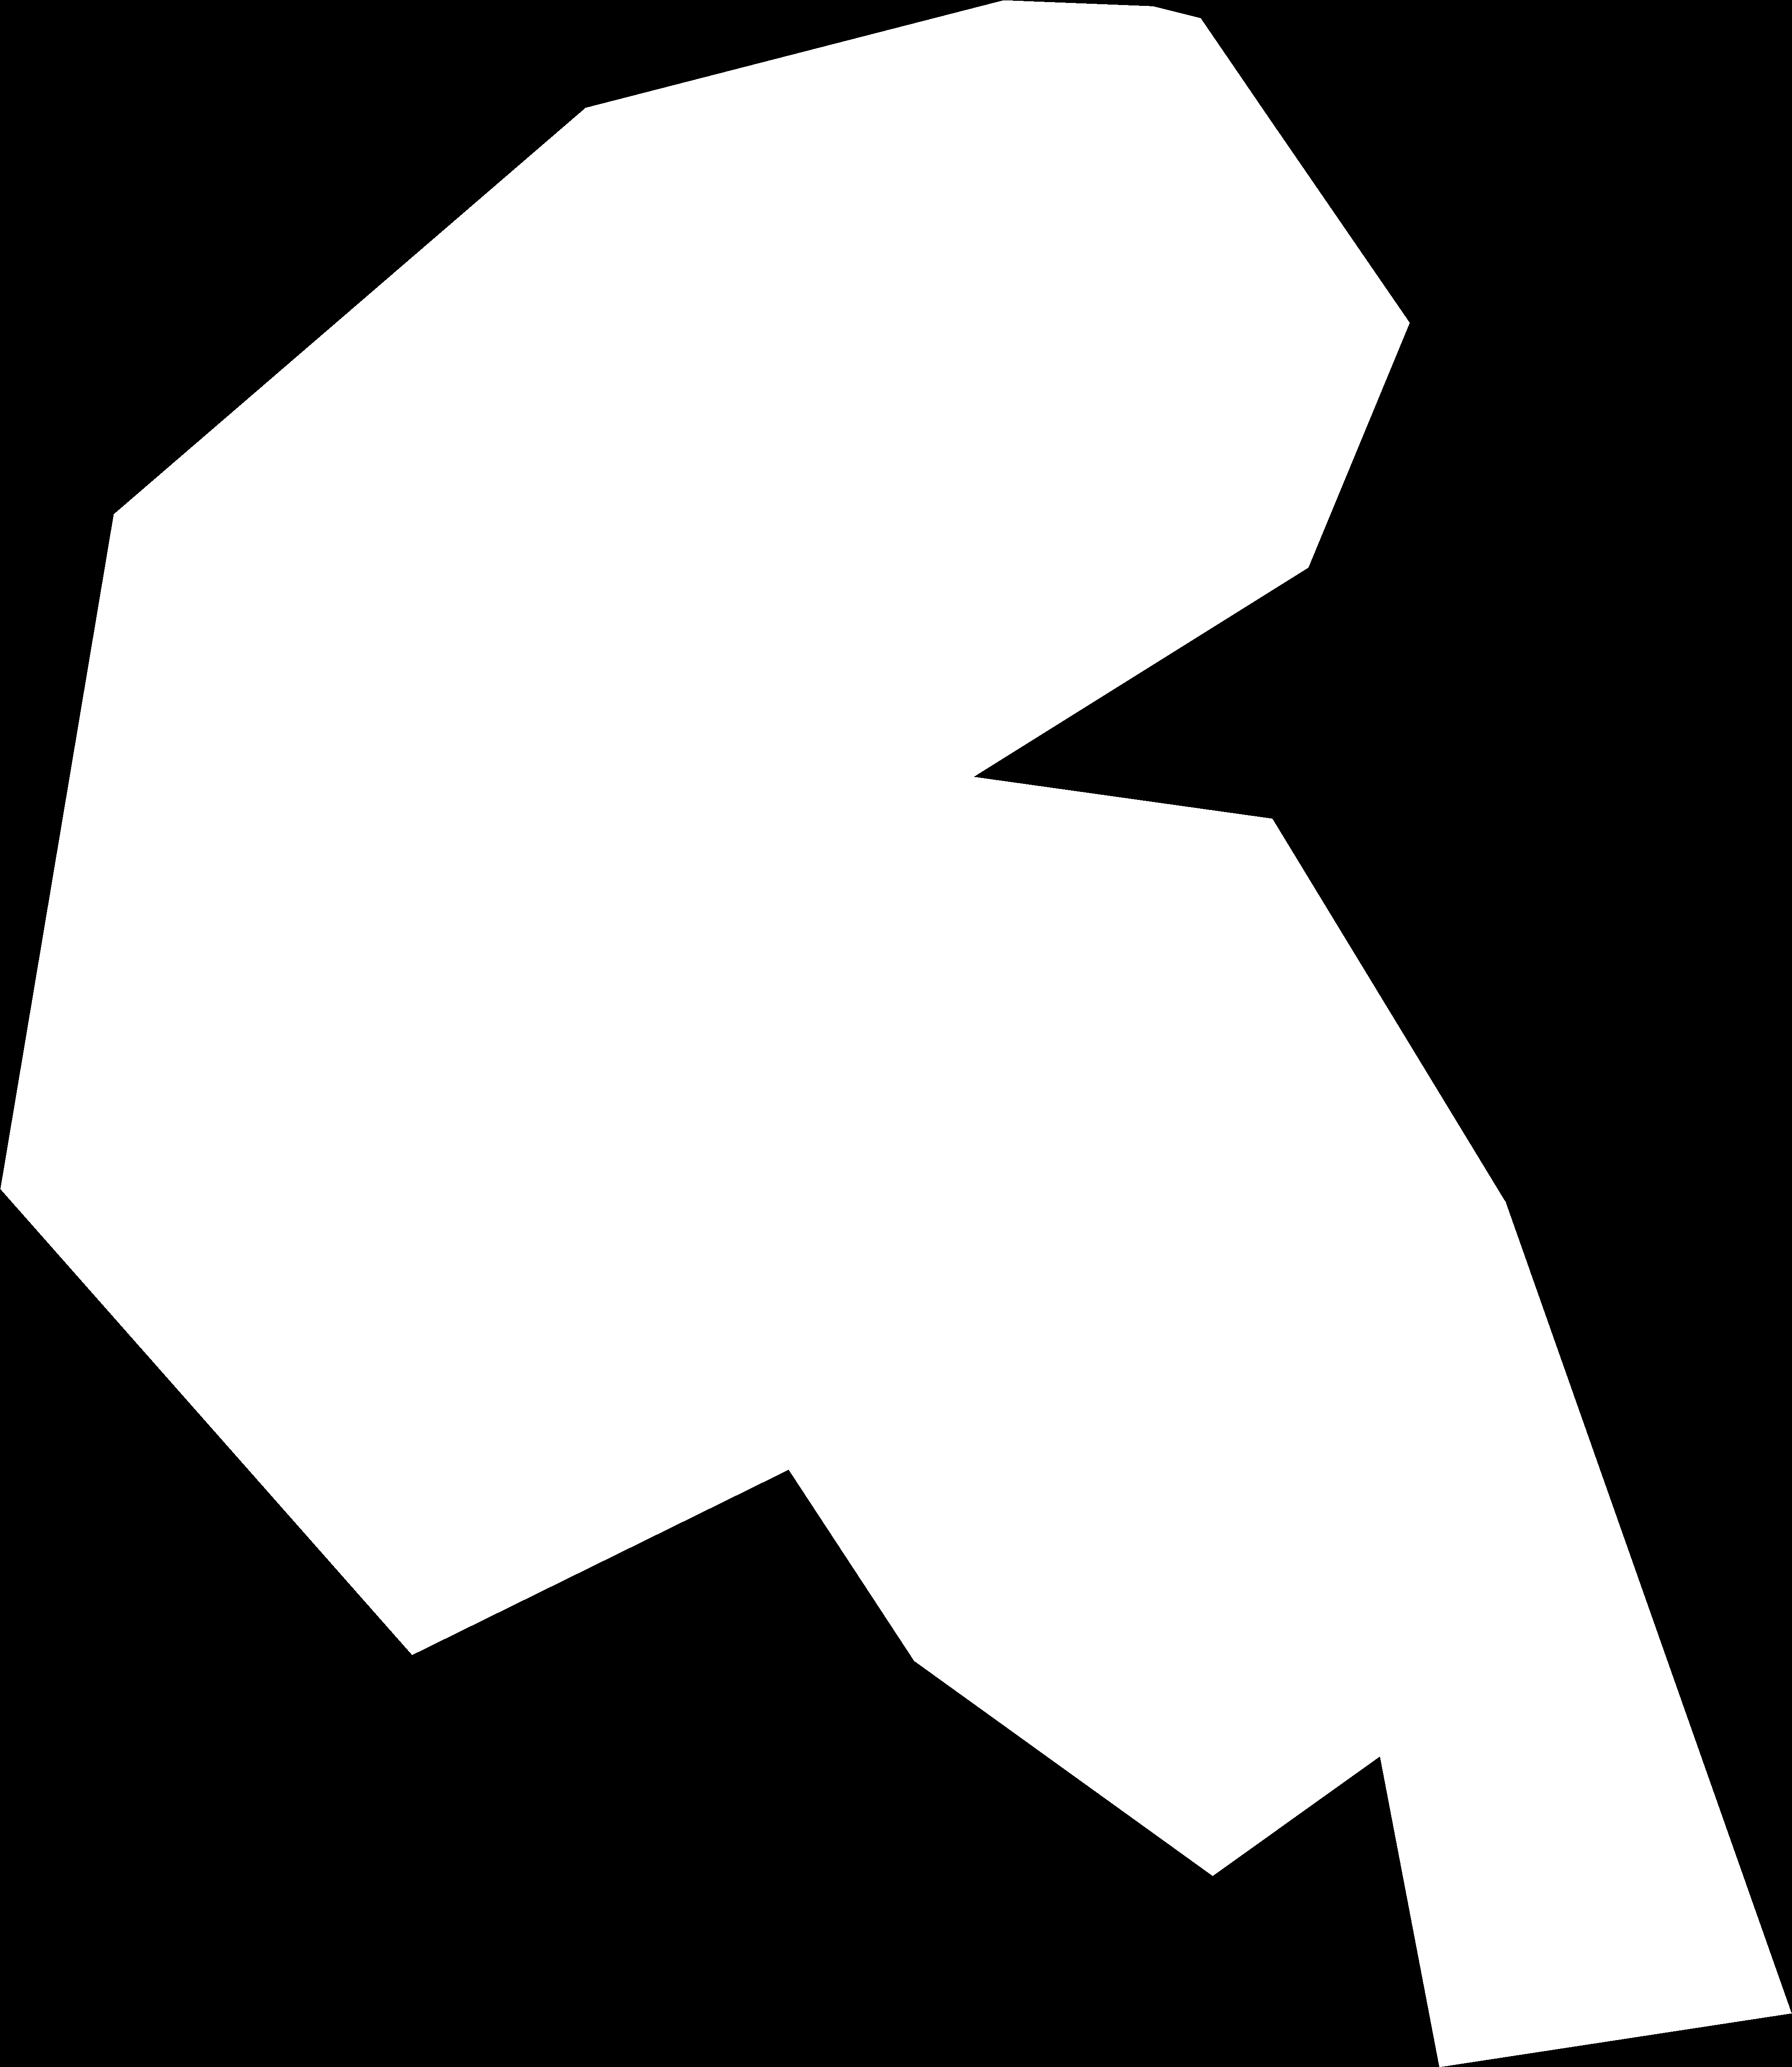
\includegraphics[width=.5\linewidth]{T001_Other_(4.00,416425,200638,17047,19660)-mask.png}
    \captionof{figure}{(package, annotation type, down-scaling factor, x, y, width, height) : T001\_Other\_(4.00,416425,
    200638,17047,19660)-mask.png}
    \label{fig:annotation}
\end{minipage}

\vspace{7mm}

\par After this, the images were processed via Python. We cut out \begin{markdown} 
`512 x 512 x 3`  
\end{markdown} 
sized patches and matched the location of the annotations to the corresponding patches, therefore, getting patch level segmentation of the whole slide image. To get rid of the meaningless patches, those that were mainly white, containing only tissue residue or scanning errors we applied pixel thresholds on the patches. We took the intensity from the HSI components (hue, saturation, and intensity) and set a threshold of 245 for 8-bit pixels to extract all the white patches. We also calculated the saturation for the patch and if it was less then .05 we said that the pixel is mainly gray, therefore useless and excluded it.

\begin{figure}[H]
    \centering
    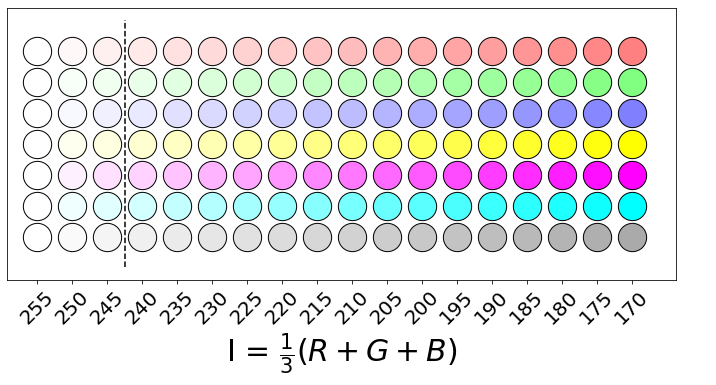
\includegraphics[width=.6\textwidth]{intensity.png}
    \caption{White limit}
    \label{fig:intensity}
\end{figure}

\begin{figure}[H]
    \centering
    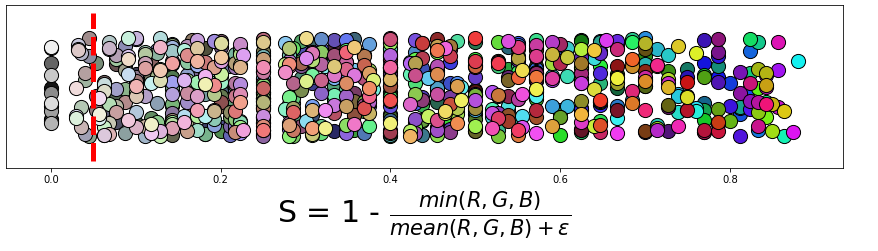
\includegraphics[width=.7\textwidth]{saturation.png}
    \captionof{figure}{Gray limit}
    \label{fig:saturation}
\end{figure}

\vspace{4mm}

\par Here I also illustrate to justify this and show the image patches acquired as a result after applying this thresholding methodology. It is obvious that the method took care of removing the residual tissue and remains of grime (dirt particles, fur, hair, etc.) on the glass plate that the slide was on.

\vspace{10mm}

\begin{minipage}[t]{0.45\textwidth}
    \centering
    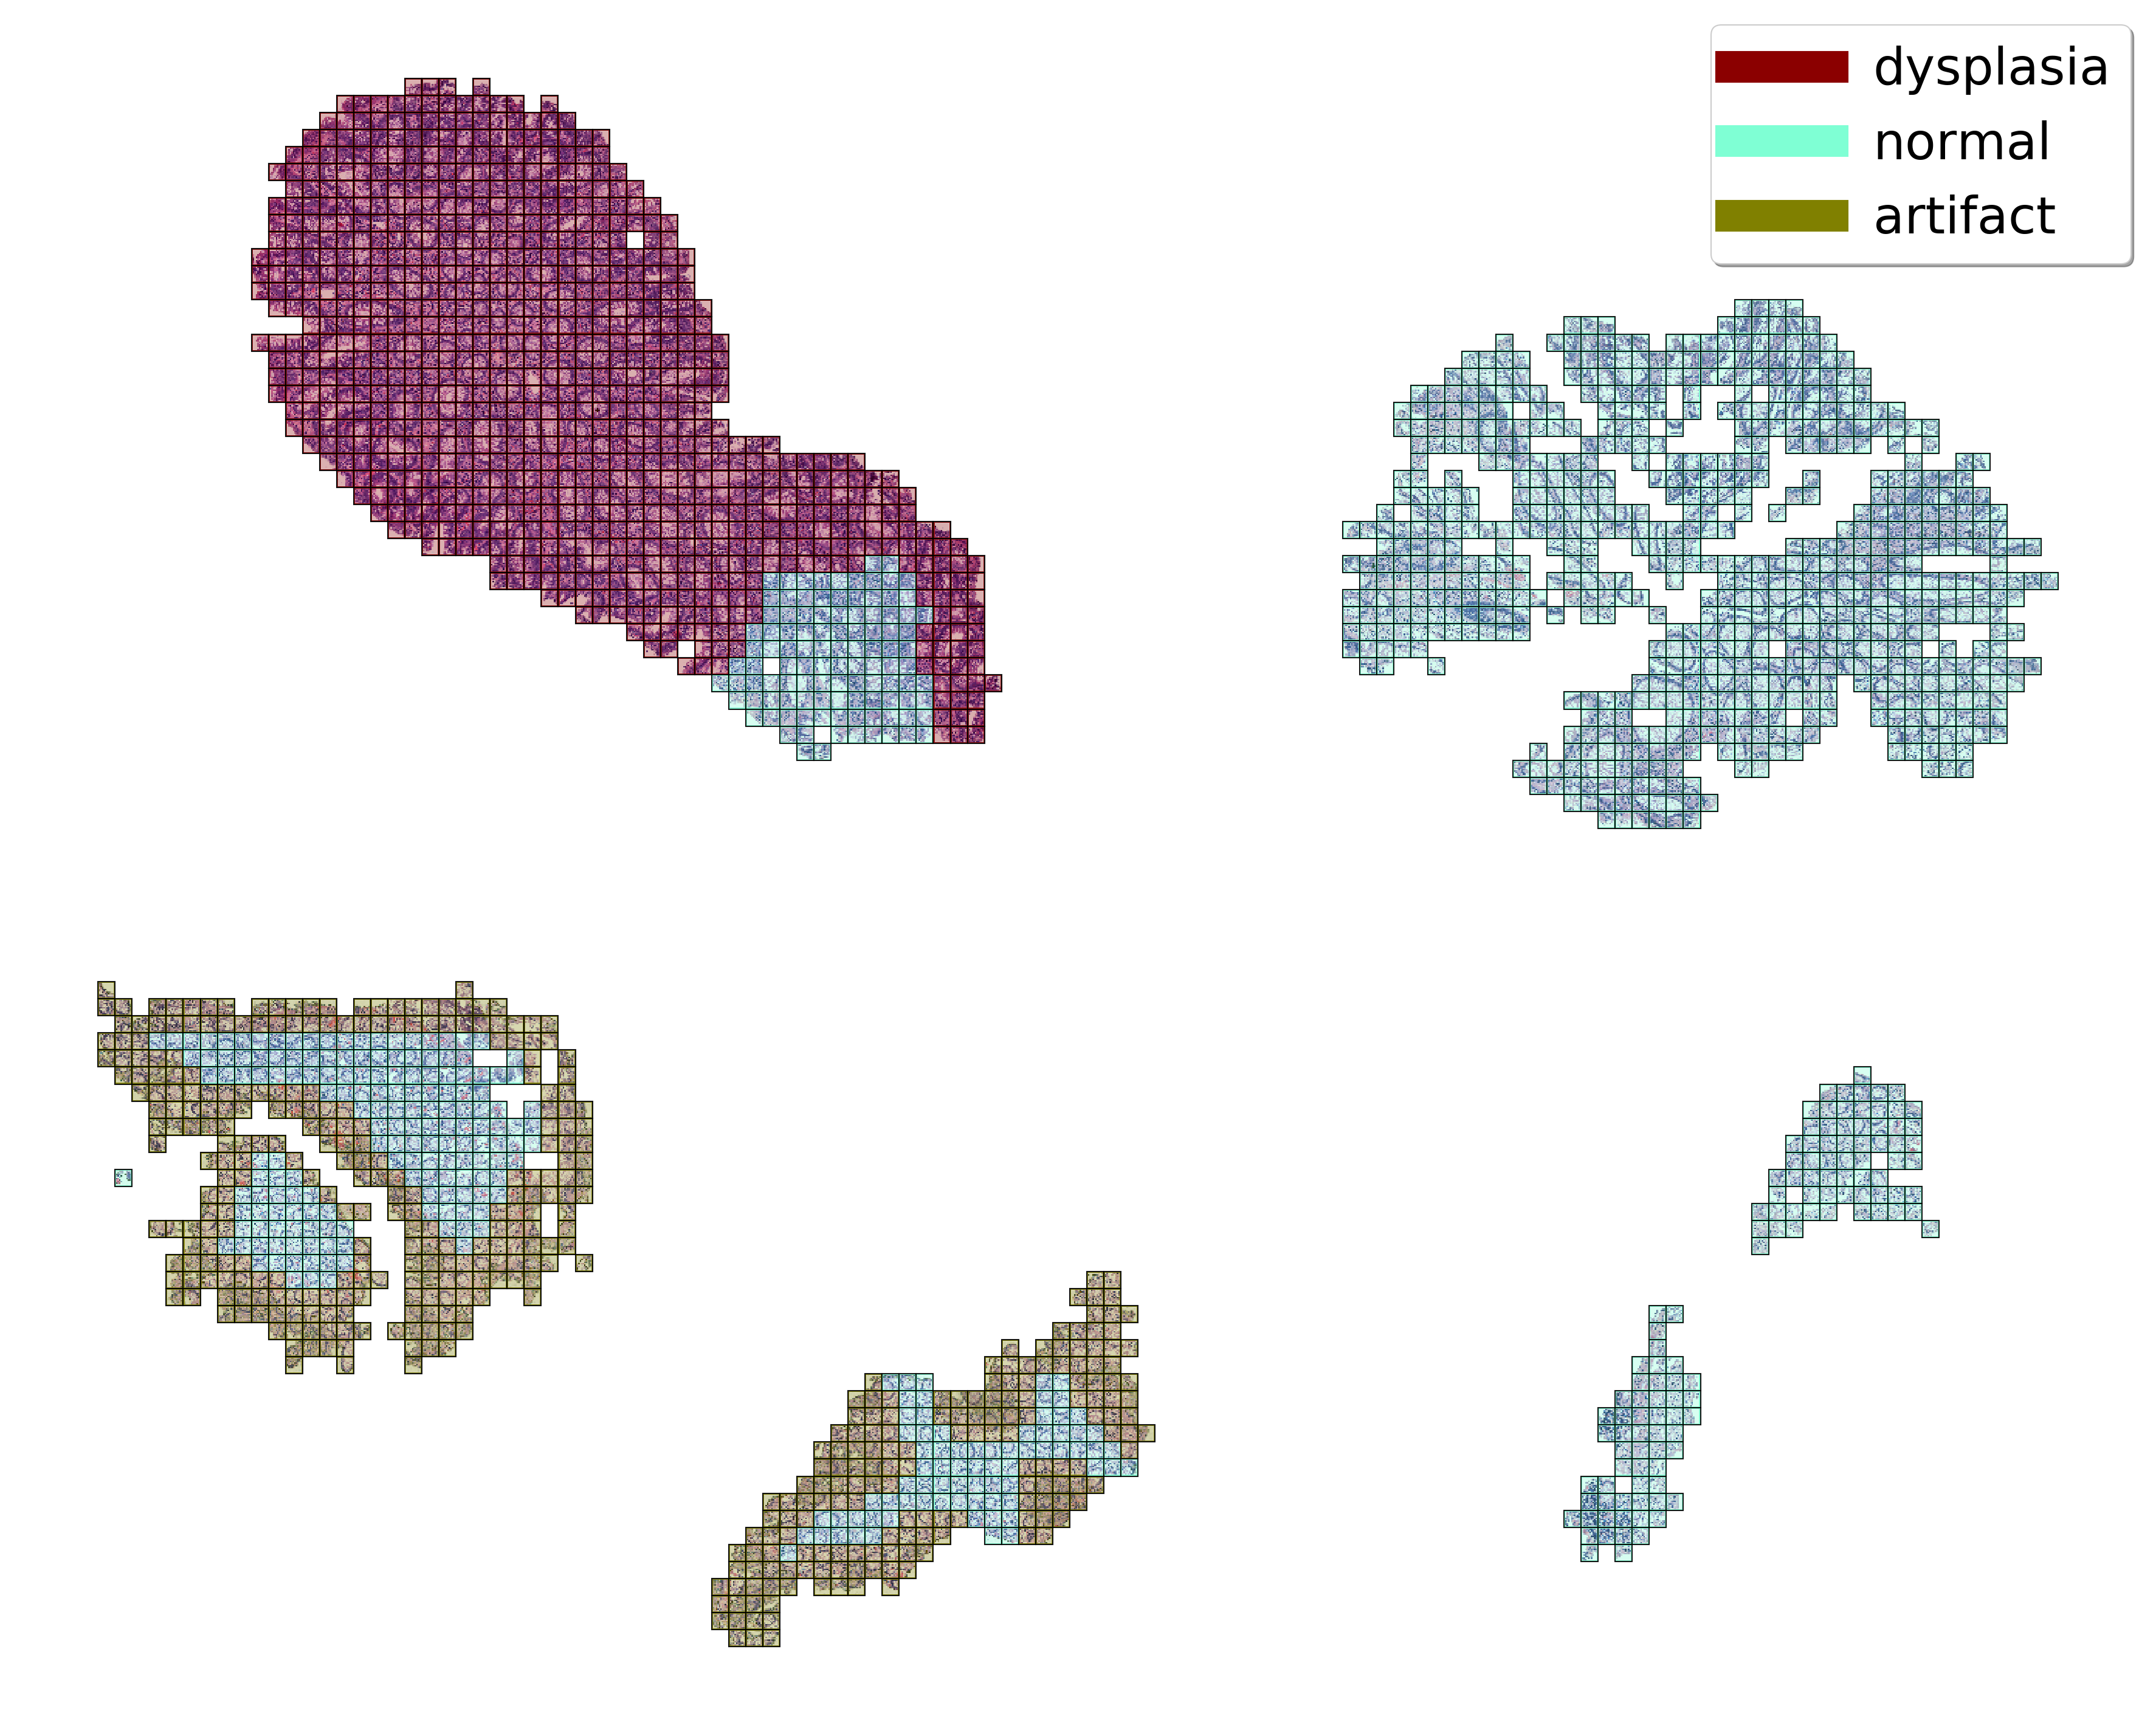
\includegraphics[width=\textwidth]{082_19_16683_zoom_1.15.png}
    \captionof{figure}{Image after thresholding and patching - with the corresponding masks on top}
    \label{fig:preprocessedslide}
\end{minipage} \qquad
\begin{minipage}[t]{0.45\textwidth}
    \centering
    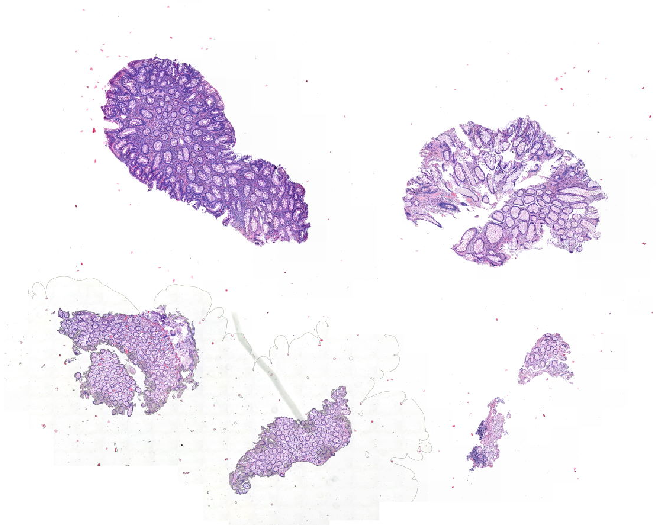
\includegraphics[width=\textwidth]{082_qupath.png}
    \captionof{figure}{The original image before the pre-processing}
    \label{fig:origslide}
\end{minipage}

\vspace{7mm}

\par The prediction process happens in two stages, the first is a patch-level classification that will be detailed later. The second process is a modified U-Net \cite{ronneberger2015u} architecture that we applied to predict a semantic segmentation map of the WSI in lower resolution. The input was a down-scaled version of the original whole slide image and each pixel was an intermediate feature from the classifier, therefore, the input contained many more channels than the usual R, G, B color channels. This had to be stored in a separate dataset and needed to be rebuilt for every classifier that we trained.

\vspace{4mm}

\subsubsection{Data for testing}

\vspace{4mm}

\par The test dataset was annotated by board-certified, expert pathologists. The annotated the slides without any additional information and got the images anonymized. They needed to record all local and global categories in checkboxes to draw a clinical conclusion and we ignored free-hand annotation as it was not crucial for comparison in clinical diagnosis. 

\vspace{4mm}

\subsubsection{Annotation categories}

\vspace{4mm}

\par We gathered two main types of annotations for the dataset: local and global labels. Locally we asked pathologists to annotate the following regions by drawing free-hand masks on the slide with QuPath. The categories were selected based on clinical relevance, expert review, and consensus.

\vspace{4mm}

\begin{enumerate}
    \item \textbf{dysplasia} - abnormal epithelial growth
    \item \textbf{highgrade\_dysplasia} - severe dysplasia (annotated inside dysplasia)
    
    \begin{minipage}[t]{0.45\textwidth}
        \centering
        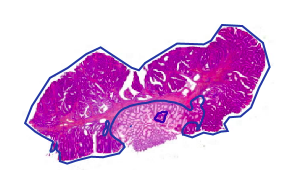
\includegraphics[width=.8\linewidth]{dysplasia.png}
        \captionof{figure}{Dysplasia}
    \end{minipage}
    \begin{minipage}[t]{0.45\textwidth}
        \centering
        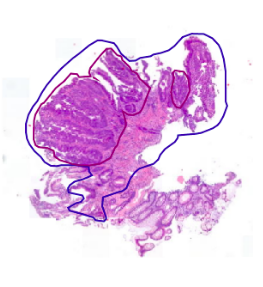
\includegraphics[width=.8\linewidth]{high_grade_dysplasia.png}
        \captionof{figure}{High-grade dysplasia}
    \end{minipage}
    
    \item \textbf{adenocarcinoma}
    \item \textbf{suspicious\_for\_invasion} - obvious signs of invasion
    \item \textbf{inflammation}
    \item \textbf{resection\_edge}
    \item \textbf{tumor\_necrosis}
    \item \textbf{lymphovascular\_invasion}
    \item \textbf{artifact}
    \item \textbf{annotated} - there are several slides present on one scan and one should be randomly selected and annotated
    
    \begin{figure}[H]
        \centering
        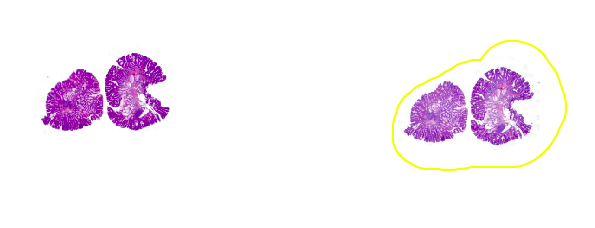
\includegraphics[width=0.6\textwidth]{annotated.png}
    \end{figure}
    
\end{enumerate}

\par Above some illustration is present with the annotated local categories. For the global labels the below list was selected:

\vspace{4mm}

\begin{itemize}
    \item main\_category
    \begin{itemize}
        \item CRC - colorectal cancer
        \item advanced\_adenoma
        \item non\_neoplastic\_leison
        \item negative
    \end{itemize}
    \item Haggit\_level \cite{aarons2014management}
    \item polyp\_type
    \begin{itemize}
        \item hyperplastic\_polyp
        \item sessile\_serrated\_polyp
        \item traditional\_serrated\_adenoma
        \item tubular\_adenoma
        \item tubulovillous\_adenoma
        \item villous\_adenoma
        \iteme hybrid
    \end{itemize}
    \item biopsy\_or\_polyp - (either biopsy or polyp, the type of the sample)
    \item other comments
\end{itemize}

\vspace{4mm}

\subsection{Vision models}

\vspace{7mm}

\par Our vision models were implemented in Tensorflow v2.0. and as I mentioned before it was a two-step process. The first model was a ResNet50 based architecture \cite{he2016deep} with a fully-connected head on top of it. Optimization was done with the Rectified Adam optimizer \cite{liu2019variance} with lookahead \cite{zhang2019lookahead}. The objective function was the sum of pairwise binary cross-entropy loss since a patch could be labeled with more categories if its on a mask edge. This model has approximately 24 million trainable parameters: 

\vspace{4mm}

\begin{table}[H]
    \centering
    \begingroup
    \setlength{\arrayrulewidth}{0.1mm}
    \setlength{\tabcolsep}{22pt}
    \renewcommand{\arraystretch}{1.7}
    \scriptsize
    \begin{tabular}{| c | c |} \hline
        \textbf{layer} name &  \textbf{ResNet50} \\ \hline
        conv1 &  \makecell{7 \times 7, 64, stride \quad 2} \\ \hline
        conv2\_x &  \makecell{3 \times 3 \quad max \quad pool, \quad stride \quad 2 \\ \begin{bmatrix}
1 \times 1, 64 \\
3 \times 3, 64 \\
1 \times 1, 256 
\end{bmatrix} \times \quad 3} \\ \hline
        conv3\_x &  \makecell{ \begin{bmatrix}
1 \times 1, 128 \\
3 \times 3, 128 \\
1 \times 1, 512 
\end{bmatrix} \times \quad 4} \\ \hline
        conv4\_x &  \makecell{ \begin{bmatrix}
1 \times 1, 256 \\
3 \times 3, 256 \\
1 \times 1, 1024 
\end{bmatrix} \times \quad 6} \\ \hline
        conv5\_x & \makecell{ \begin{bmatrix}
1 \times 1, 512 \\
3 \times 3, 512 \\
1 \times 1, 2048 
\end{bmatrix} \times \quad 3 } \\ \hline
        & average pool, 256-d fc, 128-d fc, 10-d fc \\ \hline
    \end{tabular}
    \endgroup
    \caption{Layout of the modified ResNet50 architecture - the convolutions also include batch normalization and the non-linearities are rectified linear units}
    \label{tab:my_label}
\end{table}

\vspace{4mm}

\par We applied binary cross-entropy loss between all pairs, the parameters were $10^{-4}$ base learning rate for the Rectified Adam optimizer which decayed in $45'000$ steps to $5 \cdot 10^{-6}$ while the lookahead optimizer did updates with a $0.5$ step size after six steps of exploration. 

\vspace{4mm}

\par The training was carried out on approximately 1200 training slides and the testing was done on a held-out test set of 100 randomly selected slides. After 5 epochs the training converged and a complete patch level accuracy of \textbf{73.1} \% was achieved on the held-out test set while \textbf{79.1} \% was achieved on the training set. By complete accuracy we mean a complete match between all labels of a patch, if we would have only considered naive binary accuracy these results are above \textbf{95} \% for both training and testing sets. The total process took around 3 weeks on an NVIDIA Tesla V100 16 GB GPU device.

\vspace{4mm}

\par Having trained the classification network a new training set could be built for the UNET model. This training set was assembled by taking the output of the $(128-d \ FC)$ layer of the classification network, reducing the dimension of the input patch from \begin{markdown}
512 x 512 x 3
\end{markdown}
to $128$. As it can be seen on figure \ref{fig:annotation} the annotated patches are not forming a continuous block just individual patches, therefore, we had to fill the inter-tissue regions with zeroed out 128-dimensional vectors and padded the resulting image's edges to the smallest possible power of two since the UNET does many layers of down-sampling with a \begin{markdown}
2 x 2
\end{markdown}
kernel. The resulting input feature map is therefore 

\begin{equation*}
    I_{feature\_map} = 2^{n} \cdot 2^{m} \cdot 128
\end{equation*}

\par Where $n, m$ are different based on the original extent of the annotated region on the slide. As a consequence, the segmentation model can only be trained with a batch size of 1 since each input feature is differently sized. 

\vspace{4mm}

\begin{table}[H]
    \centering
    \begin{adjustbox}{width=.7\textwidth}
    \begingroup
    \setlength{\arrayrulewidth}{0.1mm}
    \setlength{\tabcolsep}{9pt}
    \renewcommand{\arraystretch}{.5}
    \tiny
    \begin{tabular}{| c | c |} \hline
        \textbf{layer name} &  \textbf{Modified UNET} \\ \hline
        conv1 - down sampling &  \makecell{
        \begin{bmatrix}
            3 \times 3, 256
        \end{bmatrix}, stride 2, LeakyReLU} \\ \hline
        conv2 - down sampling &  \makecell{
        \begin{bmatrix}
            3 \times 3, 512
        \end{bmatrix}, stride 2, \\ InstanceNormalization, LeakyReLU} \\ \hline
        conv3 - down sampling &  \makecell{
        \begin{bmatrix}
            3 \times 3, 512
        \end{bmatrix}, stride 2, \\ InstanceNormalization, LeakyReLU} \\ \hline
        conv4\_1 - down sampling &  \makecell{
        \begin{bmatrix}
            3 \times 3, 1024
        \end{bmatrix}, stride 2, \\ InstanceNormalization, LeakyReLU} \\ \hline
        conv4\_2 - down sampling &  \makecell{
        \begin{bmatrix}
            3 \times 3, 1024
        \end{bmatrix}, stride 2, \\ InstanceNormalization, LeakyReLU} \\ \hline \hline
        %%%%%%%%%%%%%%%
        %%%%%%%%%%%%%%%
        upconv4\_1 - up sampling &  \makecell{ transpose convolution - 
        \begin{bmatrix}
            3 \times 3, 1024
        \end{bmatrix}, \\ 
        stride 2, dropout 0.5 \\ InstanceNormalization, ReLU} \\ \hline
        upconv4\_2 - up sampling &  \makecell{ transpose convolution - 
        \begin{bmatrix}
            3 \times 3, 512
        \end{bmatrix}, \\ 
        stride 2, dropout 0.5 \\ InstanceNormalization, ReLU} \\ \hline
        upconv3 - up sampling &  \makecell{ transpose convolution - 
        \begin{bmatrix}
            3 \times 3, 512
        \end{bmatrix}, \\ 
        stride 2 \\ InstanceNormalization, ReLU} \\ \hline
        upconv2 - up sampling &  \makecell{ transpose convolution - 
        \begin{bmatrix}
            3 \times 3, 256
        \end{bmatrix}, \\ 
        stride 2 \\ InstanceNormalization, ReLU} \\ \hline
        upconv1 - up sampling &  \makecell{ transpose convolution - 
        \begin{bmatrix}
            3 \times 3, 11
        \end{bmatrix}, \\ 
        stride 2 \\ InstanceNormalization, ReLU} \\ \hline
    \end{tabular}
    \endgroup
    \end{adjustbox}
    \caption{Layout of the modified UNET architecture - the appropiate skip connections have been established}
    \label{tab:unet_arch}
\end{table}

\vspace{4mm}

\par  The target feature map is an $\argmax$ taken over the true patch label. This way we drop some labels where a patch is both annotated normal and dysplasia due to being on an annotations margin but it does seem a minor issue since the original region is down-scaled by a factor of 512 where the annotation edges do not matter that much. With the zeroed out features a new target appeared and we could call it background. So in total, we have now 11 distinct and mutually exclusive labels to predict for a feature in the map, therefore it is possible to use categorical cross-entropy as our objective function.

\vspace{4mm}

\par The architecture of the modified UNET model is presented above in table \ref{tab:unet_arch} where the appropriate skip connections have been established between $(conv4\_1, upconv4\_1)$, $(conv3, upconv4\_2)$, $(conv2, upconv3)$, $(conv1, upconv2)$:

\vspace{4mm}

\begin{figure}[H]
    \centering
    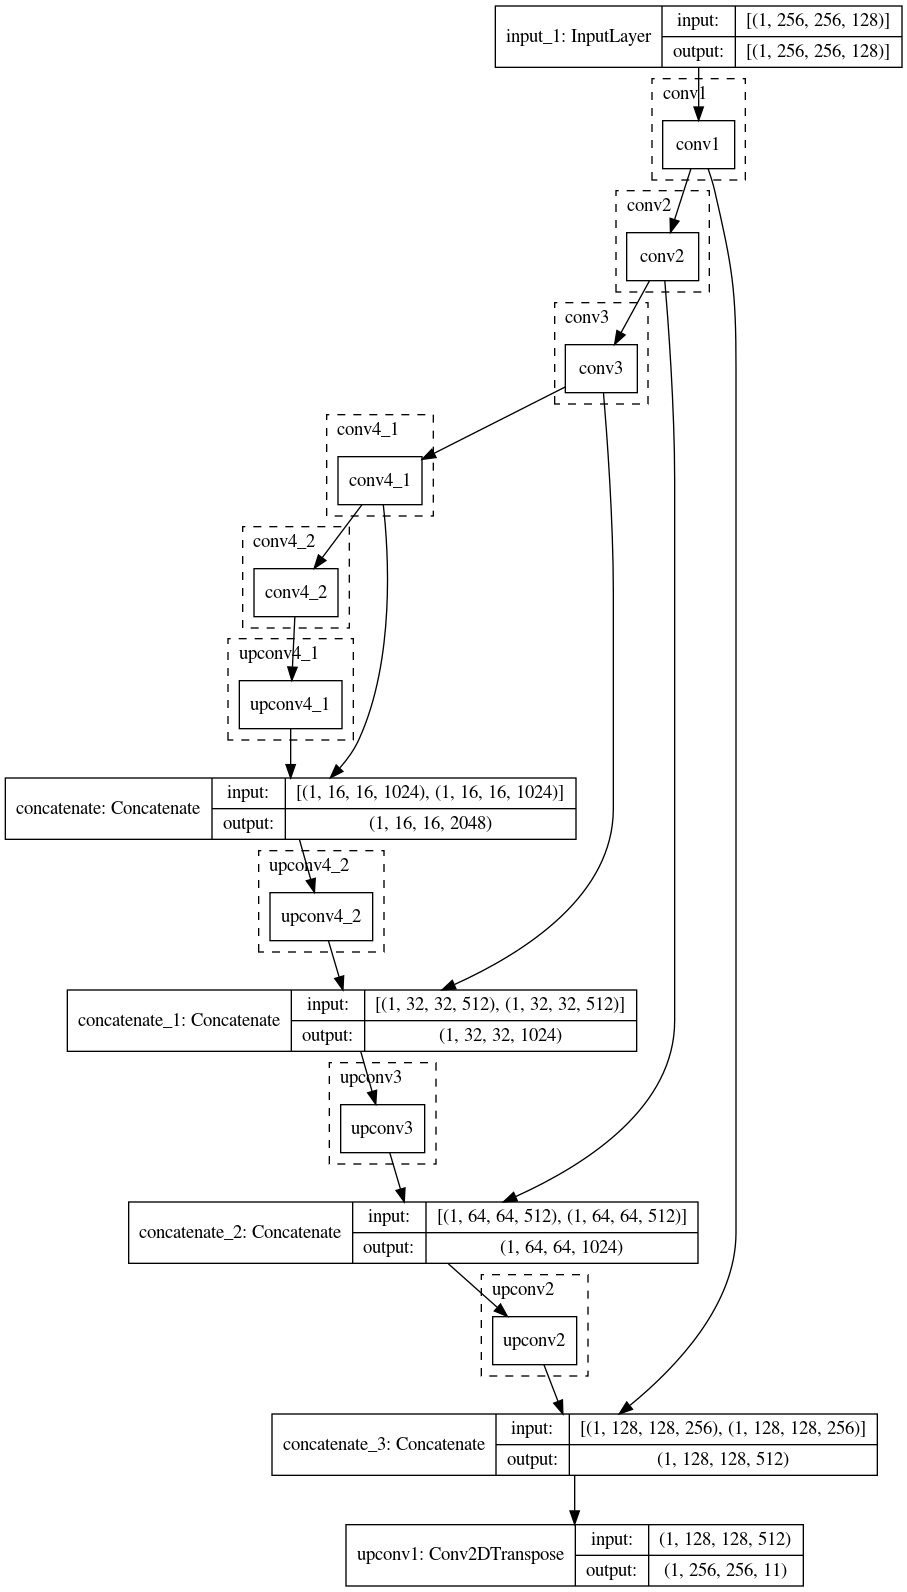
\includegraphics[width=0.6\textwidth]{model.png}
    \caption{UNET skip connections visualized}
    \label{fig:unet_skip_vis}
\end{figure}

\vspace{4mm}

\par Here an input size of  \begin{markdown}
256 x 256 x 128
\end{markdown}
was provided for simplicity, selecting $n, m$ to be both $8$. This was done to be able to see appropriate dimensions along with concatenation layers and convolutional layers. 

\vspace{4mm}

\par Training was executed for 7 epochs with early stopping, the Rectified Adam optimizer was used with Lookahead and the objective was categorical cross-entropy for the 11 labels available. Data augmentation techniques were implemented such as random cropping, horizontal and vertical flipping, and the last but not least $\pm 90^{\circ}$ rotations. The UNET model contained approximately 40 million parameters and converged after the first two epochs:

\vspace{4mm}

\begin{figure}[H]
    \centering
    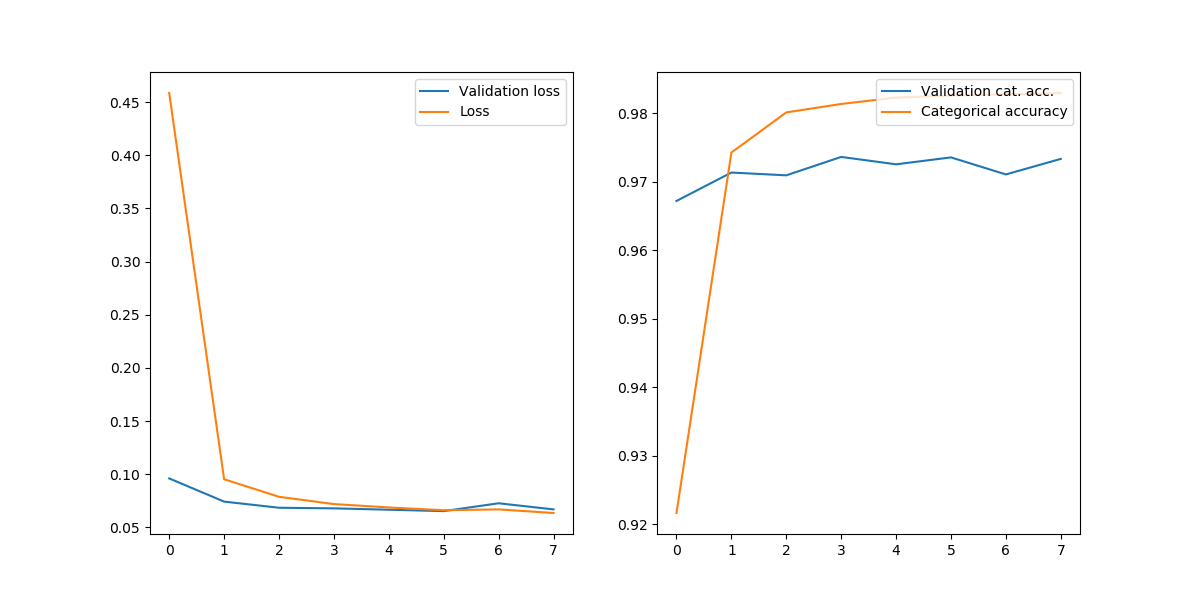
\includegraphics[width=0.85\textwidth]{results/unet_training_history.png}
    \caption{UNET training history : loss/accuracy - epoch}
    \label{fig:unet_training_history}
\end{figure}

\vspace{4mm}

\par The training was done on the same set as the training of the classification network and the testing was executed on the held-out test set as well.

\vspace{4mm}

\begin{figure}[H]
    \centering
    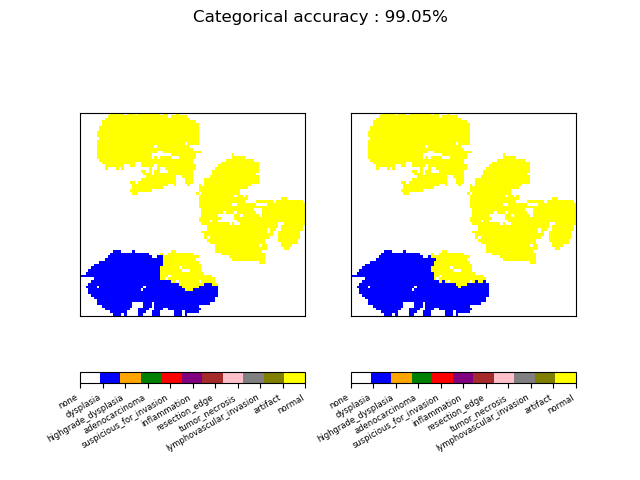
\includegraphics[width=0.62\textwidth]{results/009_19_5011_I.png}
    \caption{Detecting dysplasia and normal tissue with high accuracy}
    \label{fig:dysplasia_normal_unet}
\end{figure}

\vspace{4mm}

\par Detecting dysplasia and normal tissue seem to work well and achieve a high accuracy score in almost all cases on the test set. The categorical accuracy on top of figure \ref{fig:dysplasia_normal_unet} was taken without the background class since that is very easy to predict and would rise accuracies even higher without any further meaning. Moving on to more serious categories:

\vspace{4mm}

\begin{figure}[H]
    \centering
    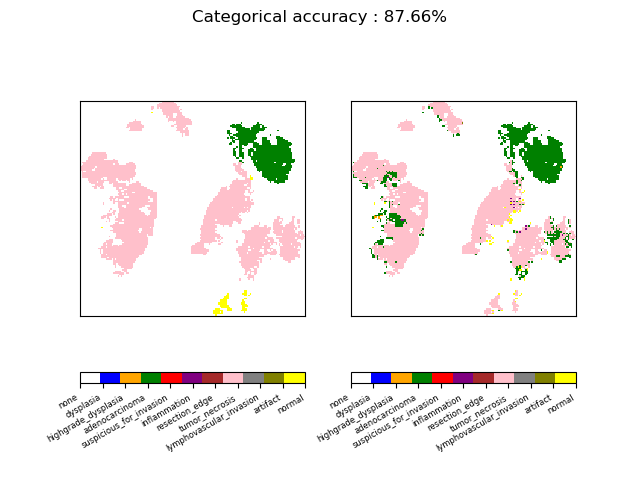
\includegraphics[width=0.75\textwidth]{results/046_19_8538.png}
    \caption{Adenocarcinoma and tumor necrosis detection with lower accuracy}
    \label{fig:adeno_tumor_unet}
\end{figure}

\vspace{4mm}

\par In figure \ref{fig:adeno_tumor_unet} we can observe that separating adenocarcinoma and tumor necrosis is not perfect and even an originally normal region has been annotated tumor necrosis in the predicted label map. They are qualitative results even though we can calculate categorical accuracy scores since it is not obvious how high the inter-observer variability in real life between doctors, so we would need a more general approach to examine the results provided by the neural networks.

\vspace{7mm}

\subsection{Evaluation of results}

\vspace{7mm}

\par How one should approach evaluating results without a ground truth? Since these slides require expert pathologists to give a diagnosis and their expert review can differ, we will evaluate by what margin, it is necessary to come up with some kind of evaluation method. First, we should check the total, unaltered consensus between each pathologist who took part in the test set evaluation and compare them to the AI pathologist. This enables us to check inter-observer variability and see whether the AI doctor is an odd-one-out or not.

\vspace{4mm}

\par Let us start with the simple example of total consensus between doctors. The evaluation of slides has been reduced to the following metric. Doctors should select all the categories that apply from the local annotations ( \begin{markdown}
`none`, `dysplasia`, `highgrade_dysplasia`, `adenocarcinoma`, 
`suspicious_for_invasion`, `inflammation`, `resection_edge`,
`tumor_necrosis`, `lymphovascular_invasion`, `artifact`, `normal`
\end{markdown} 
) and a total consensus between them means that the one-hot-encoded label vectors match completely.

\vspace{4mm}

\par Evaluation, therefore, went as follows. 15 doctors have done this checkbox style evaluation for 100 test slides and selected all the appropriate local categories present on without any surgical information or meta-data. We evaluated the features from the classification network through the UNET architecture to get a semantic segmentation map of the slide and reduced all the predicted categories to a set of labels. With the exclusion of the label \begin{markdown} `none` 
\end{markdown}
we set a threshold of $5$ \% to be the minimum region occupied by the corresponding label otherwise drop it completely. With all this in mind the resulting consensus diagram is presented below:

\vspace{4mm}

\begin{figure}[H]
    \centering
    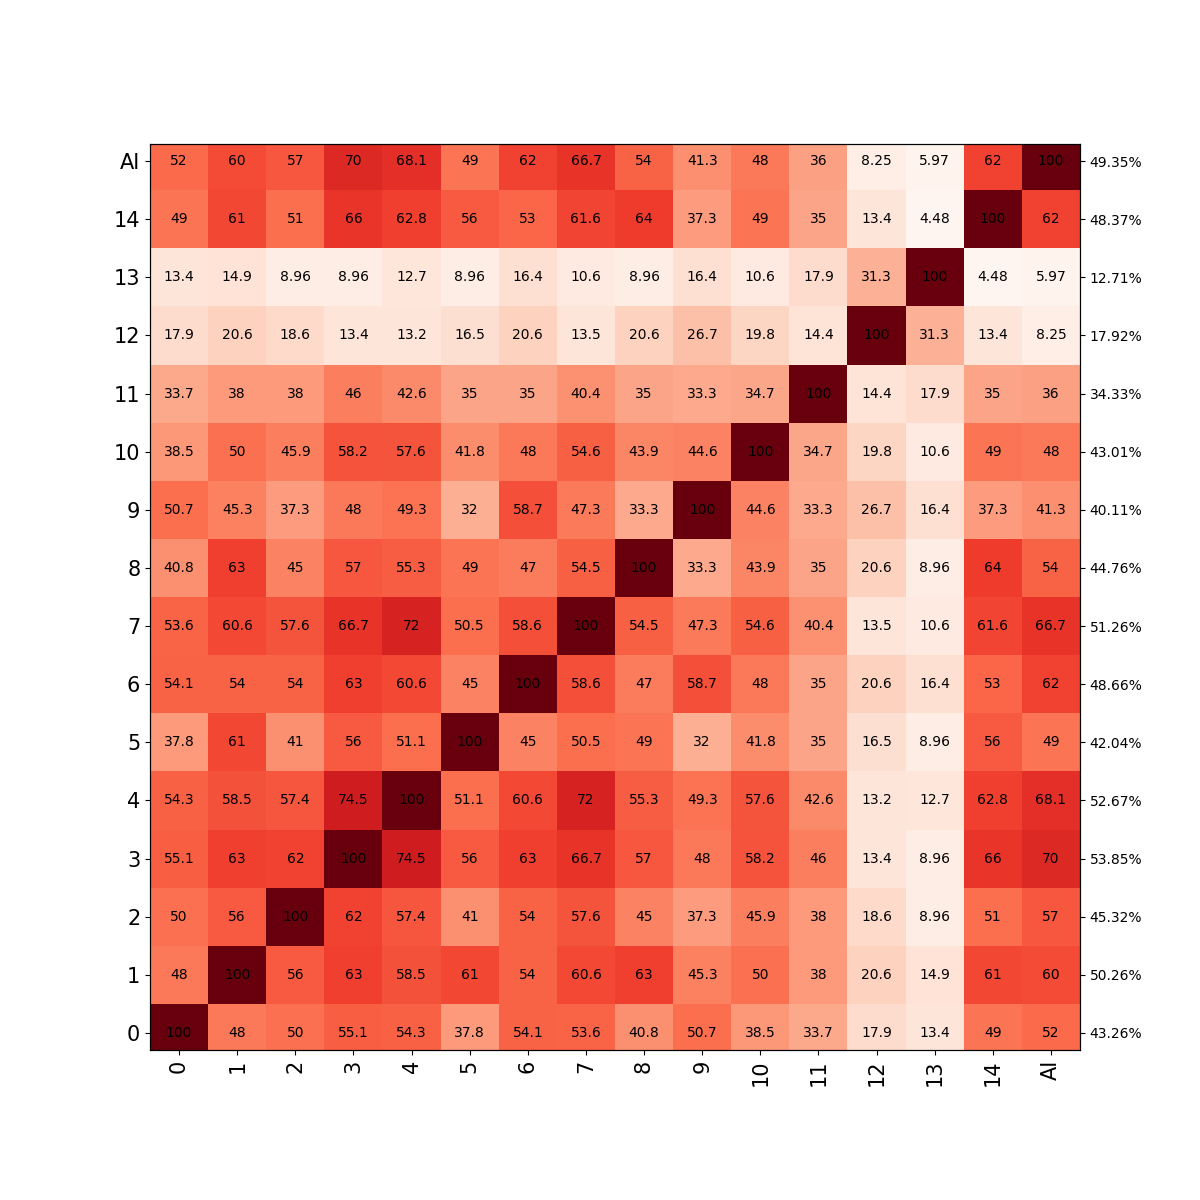
\includegraphics[width=0.9\textwidth]{results/consensus.png}
    \caption{Consensus between doctors labeled 0-14 and the AI pathologist}
    \label{fig:my_label}
\end{figure}

\vspace{4mm}

\par At the end of each row, the average of consensus scores have been taken for all pathologists with the others (excluding themselves). In this regard, the AI pathologist seems to be among the top performers. However, we should take a look at the local categories as well based on consensus to see whether the AI doctor can separate those satisfyingly.

\vspace{4mm}

\par We compared each doctor for each slide they annotated in each category. If they checked the same label for the same slide we added a score of $+1$ to that location and $+1$ for a label that they bot not included. There are some doctors who not yet annotated all the 100 test slides therefore we norm each similarity score by the matching slides. This results in very high scores in rare categories and representative similarity scores between the most important classes.

\vspace{4mm}

\begin{figure}[H]
    \centering
    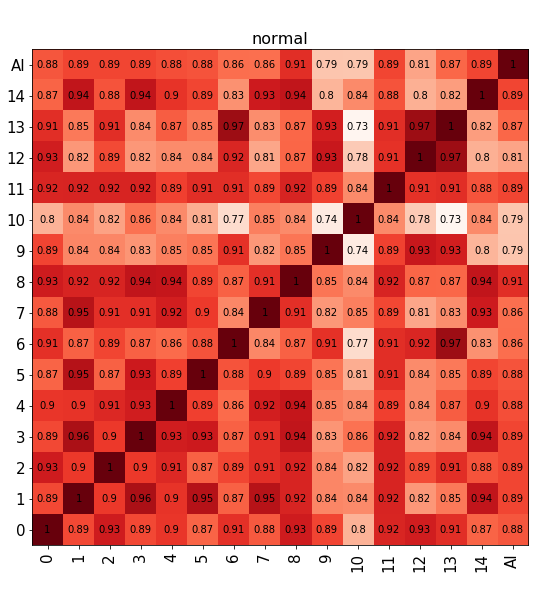
\includegraphics[width=0.8\textwidth]{results/similarities_normal.png}
    \caption{Similarities with annotating the category considered normal}
    \label{fig:sim_normal}
\end{figure}

\vspace{4mm}

\par In this category a similarity score of \textbf{86.48 \%} was achieved which is not top performance but a good average and it seems that without the outlier doctors \textbf{9, 10} this might be even further improved since the other doctors match better with their outlier colleagues on average than the AI pathologist. Below we present the categories that are mostly representative and the rest is provided in the supplementary.

\vspace{4mm}

\begin{figure}[H]
    \centering
    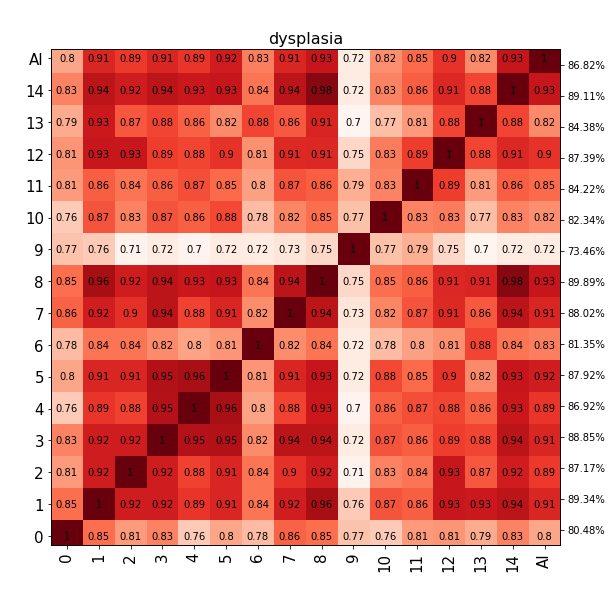
\includegraphics[width=0.7\textwidth]{results/similarities_dysplasia.png}
    \caption{Similarities with annotating the category considered dysplasia}
    \label{fig:sim_dysp}
\end{figure}

\begin{figure}[H]
    \centering
    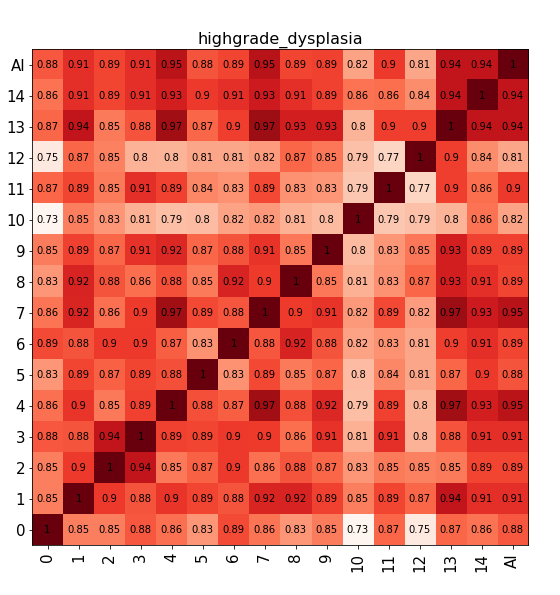
\includegraphics[width=0.7\textwidth]{results/similarities_highgrade_dysplasia.png}
    \caption{Similarities with annotating the category considered high-grade dysplasia}
    \label{fig:sim_highgradedysp}
\end{figure}

\vspace{4mm}

\par From these results it seems that both in local categories dysplasia and high-grade dysplasia the AI pathologist is performing similarly to other doctors. Sadly in a severe category such as adenocarcinoma the resulting algorithm falls behind the rest of the experts.

\begin{figure}[H]
    \centering
    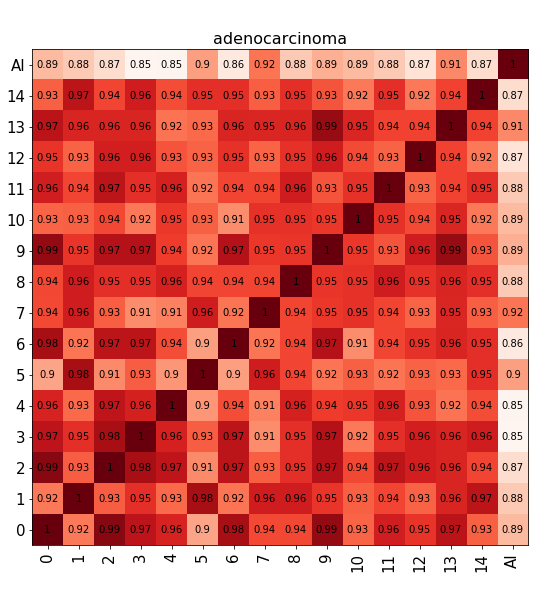
\includegraphics[width=0.8\textwidth]{results/similarities_adenocarcinoma.png}
    \caption{Similarities with annotating the category considered adenocarcinoma}
    \label{fig:sim_adeno}
\end{figure}

\vspace{4mm}

\par TODO: finish evaluation...

\newpage

\section{Deep learning for rheumatology}

\vspace{7mm}

\subsection{Overview of the problem}

\vspace{4mm}

\par Rheumatoid arthritis (RA) is an autoimmune disfunction where the immune system attacks the joints of the body and as a result they become swollen, deformed and degrade. The primary cause of the disorder is unknown and the medical care given to patients is primarily focused on reducing pain and improve life conditions. RA affects 25 million people according to \cite{vos2016global} and therefore a serious issue for the developed world.

\vspace{4mm}

\par In joints RA causes swelling and erosion of bone tissue. This can be evaluated by scanning through X-ray scans of all four limbs of a patient. A general scoring system has been proposed and implemented in clinical procedure by \cite{van1995radiographic}. It includes scoring for all joints in hand and feet for erosion and narrowing but the main aim of the authors was to develop a scoring system that helps to understand and quantify the progression of the disease in patients. The scoring involves for hands a score between 0-5 per joint for 16 joints per hand and a score between 0-4 for narrowing per joint for 15 joints per hand. The feet are scored differently for erosion since 6 joints are involved per foot and each side of the joints are score on a scale of 0-5, as for narrowing the same 6 joints are scored in 0-4 range.

\vspace{4mm}

\par This scoring is visually evaluated and an overall erosion and narrowing score is concluded from a patients hands and foot that describes the degradation rate. 

\vspace{4mm}

\begin{figure}[H]
    \centering
    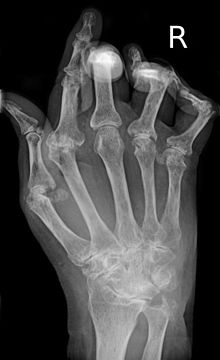
\includegraphics[width=0.3\textwidth]{ra/RheumatoideArthritisAP.jpg}
    \caption{Serious RA degradation, WikiPedia}
    \label{fig:ra_wiki}
\end{figure}

\vspace{4mm}

\subsection{The RA2-DREAM Challenge}

\vspace{4mm}

\par The problem is proposed in \url{https://www.synapse.org/#!Synapse:syn20545111/wiki/} and is still on-going at this time. As I am a challenge participant the rules apply to me and I can't share any data and result that we have on this challenge but currently we are in top three teams in all sub-challenges of the competition. I'll describe the method we used and the details from a computer vision perspective.

\vspace{4mm}

\subsection{Data}

\vspace{4mm}

\par No data can be presented before publication of the challenge paper therefore here I will not disclose any data from the challenge set. However, I need to mention that for detection we manually annotated all the challenge data for the joints with tight bounding boxes around them (~20 hours), except the wrist which contained many joints that we handled jointly. Here is a representation of bounding boxes we annotated for images found on RadioPedia:

\vspace{4mm}

\begin{minipage}[t]{0.42\textwidth}
    \centering
    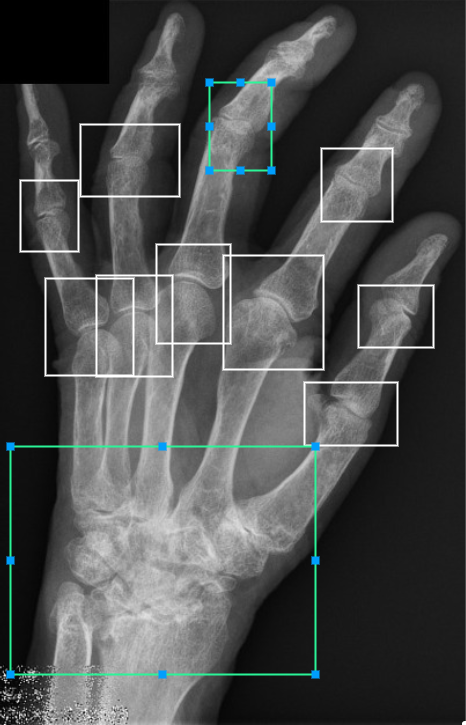
\includegraphics[width=0.6\textwidth]{ra/ra2-hand-bboxes.png}
    \captionof{figure}{Annotated hand joints for detection (image soruce - \url{https://radiopaedia.org/cases/mutilating-rheumatoid-arthritis} \url{-of-the-wrist?lang=us})}
    \label{fig:ra2-hand-annot}
\end{minipage}
\begin{minipage}[t]{0.42\textwidth}
    \centering
    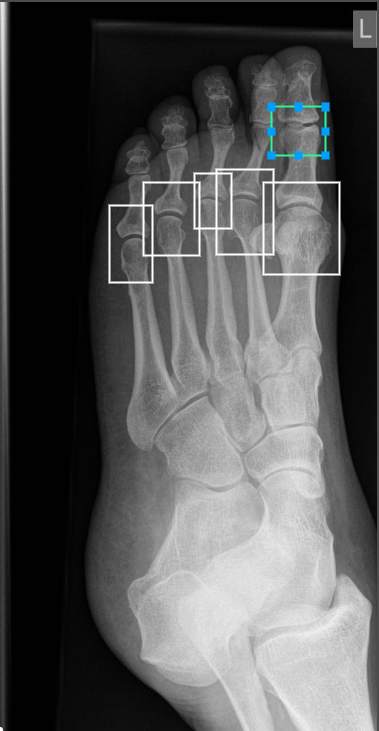
\includegraphics[width=0.6\textwidth]{ra/ra2-feet-annot.png}
    \captionof{figure}{Annotated foot joints for detection (image source - \url{https://radiopaedia.org/cases/rheumatoid-arthritis-feet?lang=us})}
    \label{fig:ra2-foot-annot}
\end{minipage}

\vspace{4mm}

\par In the challenge the annotated joints then had erosion and narrowing scores accordingly and for each patient the feet and hands were given as examples.

\vspace{4mm}

\subsection{Vision models}

\vspace{4mm}

\par In our vision models we applied a two-step approach. First we used the open-sourced FAIR Detectron2 \cite{wu2019detectron2} framework to implement a Mask-RCNN \cite{he2017mask} detection model on top of our hand-annotated data of the X-ray images. Mask-RCNN is generally used for segmentation but it is an empirical observation that using it for detection with the bounding-boxes as segmentation masks generally helps the algorithm to perform better in detection tasks.

\vspace{4mm}

\par Since the held out test set was not given to participants as the evaluation is done blindly by submitting the trained models we fit the whole training data for segmentation. Generally, selecting a reasonable number of iterations for training a detection model helps achieve good generalization and not so much over-fitting on the training set.

\vspace{4mm}

\begin{figure}[H]
    \centering
    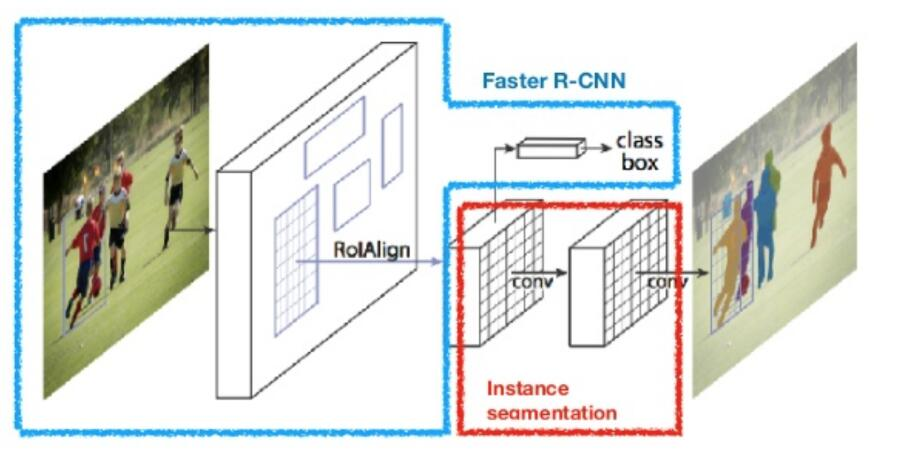
\includegraphics[width=0.6\textwidth]{ra/maskrcnn.jpg}
    \caption{A general layout of Mask-RCNN}
    \label{fig:mask-rcnn}
\end{figure}

\vspace{4mm}

\par On the above figure [\ref{fig:mask-rcnn}] the general structure of the segmentation model can be seen which a bounding box regressor based on the Faster R-CNN \cite{ren2015faster} architecture in addition with an instance segmentation module proposed in the Mask-RCNN paper.

\vspace{4mm}

\par The detection was done separately for hands and feet and we applied random horizontal flipping, brightness, saturation and contrast augmentation during the training process. Since a detection model only outputs proposals with a confidence score as results we had to select a threshold manually and had to select the most confident score for each joint. This was usually very high unless the deformation was so bad that even a human observer would have not been able to separate the joints be visual inspection. If the model would be applied in medical practice we could label the less confident segmentation results for additional medical inspection for a doctor with this method.

\vspace{4mm}

\par After the segmentation of the detected hand and foot joints we cut out the image parts from the original X-ray scans and built a dataset with joints and the corresponding erosion and narrowing scores that were given for the training data. We applied a regression model with modified ReLU activation functions that were capped at 4 and 5 according to the limit of erosion and narrowing scores for joint annotations. We applied aggressive image augmentation by changing hue, saturation, contrast levels in addition to horizontal flipping and some slight rotation of the images.

\vspace{4mm}

\par We experimented with several models such as different depth ResNet \cite{he2016deep} architectures as well as state-of-the-art EfficientNetB7 \cite{tan2019efficientnet} architecture. At last, an ensemble of these models provided the best results that we optimized jointly for root mean squared error score. Separate models were trained for hand digits, wrist and foot regression for erosion and narrowing scoring.

\newpage

\bibliographystyle{unsrt}
\bibliography{references}

\end{document}\grid
